\documentclass[oneside]{book}
\usepackage{lmodern}
\usepackage{setspace}
\setstretch{1.15}
\usepackage{amssymb,amsmath}
\usepackage{ifxetex,ifluatex}
\usepackage{fixltx2e} % provides \textsubscript
\ifnum 0\ifxetex 1\fi\ifluatex 1\fi=0 % if pdftex
  \usepackage[T1]{fontenc}
  \usepackage[utf8]{inputenc}
\else % if luatex or xelatex
  \ifxetex
    \usepackage{mathspec}
  \else
    \usepackage{fontspec}
  \fi
  \defaultfontfeatures{Ligatures=TeX,Scale=MatchLowercase}
\fi
% use upquote if available, for straight quotes in verbatim environments
\IfFileExists{upquote.sty}{\usepackage{upquote}}{}
% use microtype if available
\IfFileExists{microtype.sty}{%
\usepackage[]{microtype}
\UseMicrotypeSet[protrusion]{basicmath} % disable protrusion for tt fonts
}{}
\PassOptionsToPackage{hyphens}{url} % url is loaded by hyperref
\usepackage[unicode=true]{hyperref}
\PassOptionsToPackage{usenames,dvipsnames}{color} % color is loaded by hyperref
\hypersetup{
            pdftitle={Blueberries in My Salad},
            pdfauthor={Amit Arora},
            colorlinks=true,
            linkcolor=NavyBlue,
            citecolor=Blue,
            urlcolor=Blue,
            breaklinks=true}
\urlstyle{same}  % don't use monospace font for urls
\usepackage{longtable,booktabs}
% Fix footnotes in tables (requires footnote package)
\IfFileExists{footnote.sty}{\usepackage{footnote}\makesavenoteenv{long table}}{}
\usepackage{graphicx,grffile}
\makeatletter
\def\maxwidth{\ifdim\Gin@nat@width>\linewidth\linewidth\else\Gin@nat@width\fi}
\def\maxheight{\ifdim\Gin@nat@height>\textheight\textheight\else\Gin@nat@height\fi}
\makeatother
% Scale images if necessary, so that they will not overflow the page
% margins by default, and it is still possible to overwrite the defaults
% using explicit options in \includegraphics[width, height, ...]{}
\setkeys{Gin}{width=\maxwidth,height=\maxheight,keepaspectratio}
% Make links footnotes instead of hotlinks:
\renewcommand{\href}[2]{#2\footnote{\url{#1}}}
\IfFileExists{parskip.sty}{%
\usepackage{parskip}
}{% else
\setlength{\parindent}{0pt}
\setlength{\parskip}{6pt plus 2pt minus 1pt}
}
\setlength{\emergencystretch}{3em}  % prevent overfull lines
\providecommand{\tightlist}{%
  \setlength{\itemsep}{0pt}\setlength{\parskip}{0pt}}
\setcounter{secnumdepth}{5}
% Redefines (sub)paragraphs to behave more like sections
\ifx\paragraph\undefined\else
\let\oldparagraph\paragraph
\renewcommand{\paragraph}[1]{\oldparagraph{#1}\mbox{}}
\fi
\ifx\subparagraph\undefined\else
\let\oldsubparagraph\subparagraph
\renewcommand{\subparagraph}[1]{\oldsubparagraph{#1}\mbox{}}
\fi

% set default figure placement to htbp
\makeatletter
\def\fps@figure{htbp}
\makeatother

\usepackage{amsmath}
\usepackage{booktabs}
\usepackage{caption}
\usepackage{longtable}

\title{Blueberries in My Salad}
\author{Amit Arora}
\date{September 2020}

\begin{document}
\maketitle

{
\hypersetup{linkcolor=black}
\setcounter{tocdepth}{1}
\tableofcontents
}
\begin{verbatim}
## Parsed with column specification:
## cols(
##   Date = col_character(),
##   Weight = col_character(),
##   BMI = col_character(),
##   `Body Fat` = col_character(),
##   `Lean Mass` = col_character(),
##   `Muscle Percentage` = col_character(),
##   `Water Percentage` = col_character()
## )
\end{verbatim}

\begin{verbatim}
## Warning: Problem with `mutate()` input `Date`.
## x  2 failed to parse.
## i Input `Date` is `ymd(Date)`.
\end{verbatim}

\begin{verbatim}
## Warning: 2 failed to parse.
\end{verbatim}

\begin{verbatim}
## Parsed with column specification:
## cols(
##   Date = col_character(),
##   Weight = col_character(),
##   BMI = col_character(),
##   `Body Fat` = col_character(),
##   `Lean Mass` = col_character(),
##   `Muscle Percentage` = col_character(),
##   `Water Percentage` = col_character()
## )
\end{verbatim}

\begin{verbatim}
## Warning: Problem with `mutate()` input `Date`.
## x  2 failed to parse.
## i Input `Date` is `ymd(Date)`.

## Warning:  2 failed to parse.
\end{verbatim}

\begin{verbatim}
## Warning: attributes are not identical across measure variables;
## they will be dropped
\end{verbatim}

\begin{verbatim}
## NULL
\end{verbatim}

\begin{verbatim}
## INFO [2020-09-12 17:54:33] params used:
## START_DATE=2020-02-17,
## DATA_DIR=data,
## P1_NAME=Nidhi,
## P2_NAME=Amit,
## P1_DATA_URL=https://raw.githubusercontent.com/aarora79/biomettracker/master/data/Nidhi.csv,
## P2_DATA_URL=https://raw.githubusercontent.com/aarora79/biomettracker/master/data/Amit.csv,
## CAPTION=Source: Daily measurements done @home,
## IMPORTANT_DATES_FPATH=https://raw.githubusercontent.com/aarora79/biomettracker/master/data/important_dates.csv,
## NUDGE_X=1,
## NUDGE_Y=5,
## P1_TARGET_WEIGHT=128,
## P1_WEIGHT_CAP=160,
## P1_WEIGHT_FLOOR=120,
## P2_TARGET_WEIGHT=190,
## P2_WEIGHT_CAP=260,
## P2_WEIGHT_FLOOR=180
\end{verbatim}

\begin{verbatim}
## Parsed with column specification:
## cols(
##   Date = col_character(),
##   Weight = col_character(),
##   BMI = col_character(),
##   `Body Fat` = col_character(),
##   `Lean Mass` = col_character(),
##   `Muscle Percentage` = col_character(),
##   `Water Percentage` = col_character()
## )
\end{verbatim}

\begin{verbatim}
## Warning: Problem with `mutate()` input `Date`.
## x  2 failed to parse.
## i Input `Date` is `ymd(Date)`.
\end{verbatim}

\begin{verbatim}
## Warning: 2 failed to parse.
\end{verbatim}

\begin{verbatim}
## INFO [2020-09-12 17:54:33] read data for Nidhi from https://raw.githubusercontent.com/aarora79/biomettracker/master/data/Nidhi.csv, shape of dataframe=240x8
\end{verbatim}

\begin{verbatim}
## INFO [2020-09-12 17:54:33] c(18309, 18310, 18311, 18312, 18313, 18315)
## INFO [2020-09-12 17:54:33] c("151.9", "150.36", "149.69", "148.81", "147.49", "148.37")
## INFO [2020-09-12 17:54:33] c("28.0", "27.7", "27.5", "27.4", "27.1", "27.3")
## INFO [2020-09-12 17:54:33] c("32.3", "32.0", "31.8", "31.7", "31.4", "31.5")
## INFO [2020-09-12 17:54:33] c("102.84", "102.24", "102.09", "101.64", "101.18", "101.63")
## INFO [2020-09-12 17:54:33] c("32.0", "32.1", "32.1", "32.1", "32.2", "32.2")
## INFO [2020-09-12 17:54:33] c("49.4", "49.7", "49.8", "49.9", "50.1", "50.0")
## INFO [2020-09-12 17:54:33] c("Nidhi", "Nidhi", "Nidhi", "Nidhi", "Nidhi", "Nidhi")
\end{verbatim}

\begin{verbatim}
## INFO [2020-09-12 17:54:33] Min.   :2020-02-17  
## INFO [2020-09-12 17:54:33] 1st Qu.:2020-04-10  
## INFO [2020-09-12 17:54:33] Median :2020-06-03  
## INFO [2020-09-12 17:54:33] Mean   :2020-05-31  
## INFO [2020-09-12 17:54:33] 3rd Qu.:2020-07-23  
## INFO [2020-09-12 17:54:33] Max.   :2020-09-08  
## INFO [2020-09-12 17:54:33] Length:240        
## INFO [2020-09-12 17:54:33] Class :character  
## INFO [2020-09-12 17:54:33] Mode  :character  
## INFO [2020-09-12 17:54:33] NA
## INFO [2020-09-12 17:54:33] NA
## INFO [2020-09-12 17:54:33] NA
## INFO [2020-09-12 17:54:33] Length:240        
## INFO [2020-09-12 17:54:33] Class :character  
## INFO [2020-09-12 17:54:33] Mode  :character  
## INFO [2020-09-12 17:54:33] NA
## INFO [2020-09-12 17:54:33] NA
## INFO [2020-09-12 17:54:33] NA
## INFO [2020-09-12 17:54:33] Length:240        
## INFO [2020-09-12 17:54:33] Class :character  
## INFO [2020-09-12 17:54:33] Mode  :character  
## INFO [2020-09-12 17:54:33] NA
## INFO [2020-09-12 17:54:33] NA
## INFO [2020-09-12 17:54:33] NA
## INFO [2020-09-12 17:54:33] Length:240        
## INFO [2020-09-12 17:54:33] Class :character  
## INFO [2020-09-12 17:54:33] Mode  :character  
## INFO [2020-09-12 17:54:33] NA
## INFO [2020-09-12 17:54:33] NA
## INFO [2020-09-12 17:54:33] NA
## INFO [2020-09-12 17:54:33] Length:240        
## INFO [2020-09-12 17:54:33] Class :character  
## INFO [2020-09-12 17:54:33] Mode  :character  
## INFO [2020-09-12 17:54:33] NA
## INFO [2020-09-12 17:54:33] NA
## INFO [2020-09-12 17:54:33] NA
## INFO [2020-09-12 17:54:33] Length:240        
## INFO [2020-09-12 17:54:33] Class :character  
## INFO [2020-09-12 17:54:33] Mode  :character  
## INFO [2020-09-12 17:54:33] NA
## INFO [2020-09-12 17:54:33] NA
## INFO [2020-09-12 17:54:33] NA
## INFO [2020-09-12 17:54:33] Length:240        
## INFO [2020-09-12 17:54:33] Class :character  
## INFO [2020-09-12 17:54:33] Mode  :character  
## INFO [2020-09-12 17:54:33] NA
## INFO [2020-09-12 17:54:33] NA
## INFO [2020-09-12 17:54:33] NA
\end{verbatim}

\begin{verbatim}
## Parsed with column specification:
## cols(
##   Date = col_character(),
##   Weight = col_character(),
##   BMI = col_character(),
##   `Body Fat` = col_character(),
##   `Lean Mass` = col_character(),
##   `Muscle Percentage` = col_character(),
##   `Water Percentage` = col_character()
## )
\end{verbatim}

\begin{verbatim}
## Warning: Problem with `mutate()` input `Date`.
## x  2 failed to parse.
## i Input `Date` is `ymd(Date)`.

## Warning:  2 failed to parse.
\end{verbatim}

\begin{verbatim}
## INFO [2020-09-12 17:54:33] read data for Amit from https://raw.githubusercontent.com/aarora79/biomettracker/master/data/Amit.csv, shape of dataframe=220x8
## INFO [2020-09-12 17:54:33] c(18309, 18310, 18311, 18312, 18313, 18314)
## INFO [2020-09-12 17:54:33] c("251.33", "248.02", "247.36", "246.48", "246.03", "245.6")
## INFO [2020-09-12 17:54:33] c("38.1", "37.6", "37.5", "37.4", "37.3", "37.2")
## INFO [2020-09-12 17:54:33] c("35.9", "35.5", "35.5", "35.4", "35.3", "35.3")
## INFO [2020-09-12 17:54:33] c("161.1", "159.97", "159.55", "159.22", "159.18", "158.9")
## INFO [2020-09-12 17:54:33] c("35.6", "35.8", "35.8", "35.8", "35.8", "35.9")
## INFO [2020-09-12 17:54:33] c("46.8", "47.1", "47.1", "47.2", "47.2", "47.2")
## INFO [2020-09-12 17:54:33] c("Amit", "Amit", "Amit", "Amit", "Amit", "Amit")
## INFO [2020-09-12 17:54:33] Min.   :2020-02-17  
## INFO [2020-09-12 17:54:33] 1st Qu.:2020-04-09  
## INFO [2020-09-12 17:54:33] Median :2020-05-30  
## INFO [2020-09-12 17:54:33] Mean   :2020-05-28  
## INFO [2020-09-12 17:54:33] 3rd Qu.:2020-07-15  
## INFO [2020-09-12 17:54:33] Max.   :2020-09-08  
## INFO [2020-09-12 17:54:33] Length:220        
## INFO [2020-09-12 17:54:33] Class :character  
## INFO [2020-09-12 17:54:33] Mode  :character  
## INFO [2020-09-12 17:54:33] NA
## INFO [2020-09-12 17:54:33] NA
## INFO [2020-09-12 17:54:33] NA
## INFO [2020-09-12 17:54:33] Length:220        
## INFO [2020-09-12 17:54:33] Class :character  
## INFO [2020-09-12 17:54:33] Mode  :character  
## INFO [2020-09-12 17:54:33] NA
## INFO [2020-09-12 17:54:33] NA
## INFO [2020-09-12 17:54:33] NA
## INFO [2020-09-12 17:54:33] Length:220        
## INFO [2020-09-12 17:54:33] Class :character  
## INFO [2020-09-12 17:54:33] Mode  :character  
## INFO [2020-09-12 17:54:33] NA
## INFO [2020-09-12 17:54:33] NA
## INFO [2020-09-12 17:54:33] NA
## INFO [2020-09-12 17:54:33] Length:220        
## INFO [2020-09-12 17:54:33] Class :character  
## INFO [2020-09-12 17:54:33] Mode  :character  
## INFO [2020-09-12 17:54:33] NA
## INFO [2020-09-12 17:54:33] NA
## INFO [2020-09-12 17:54:33] NA
## INFO [2020-09-12 17:54:33] Length:220        
## INFO [2020-09-12 17:54:33] Class :character  
## INFO [2020-09-12 17:54:33] Mode  :character  
## INFO [2020-09-12 17:54:33] NA
## INFO [2020-09-12 17:54:33] NA
## INFO [2020-09-12 17:54:33] NA
## INFO [2020-09-12 17:54:33] Length:220        
## INFO [2020-09-12 17:54:33] Class :character  
## INFO [2020-09-12 17:54:33] Mode  :character  
## INFO [2020-09-12 17:54:33] NA
## INFO [2020-09-12 17:54:33] NA
## INFO [2020-09-12 17:54:33] NA
## INFO [2020-09-12 17:54:33] Length:220        
## INFO [2020-09-12 17:54:33] Class :character  
## INFO [2020-09-12 17:54:33] Mode  :character  
## INFO [2020-09-12 17:54:33] NA
## INFO [2020-09-12 17:54:33] NA
## INFO [2020-09-12 17:54:33] NA
\end{verbatim}

\begin{verbatim}
## Parsed with column specification:
## cols(
##   label = col_character(),
##   Date = col_date(format = ""),
##   include = col_logical(),
##   name = col_character()
## )
\end{verbatim}

\begin{verbatim}
## INFO [2020-09-12 17:54:33] read data for important dates from https://raw.githubusercontent.com/aarora79/biomettracker/master/data/important_dates.csv,
## shape of dataframe=17x4
## INFO [2020-09-12 17:54:33] c("Nidhi's Birthday", "Aadit's Birthday", "Nidhi's Birthday", "Aadit's Birthday", "Start training 4 days a week", "Start training 4 days a week")
## INFO [2020-09-12 17:54:33] c(18380, 18409, 18380, 18409, 18382, 18382)
## INFO [2020-09-12 17:54:33] c(FALSE, FALSE, TRUE, FALSE, TRUE, TRUE)
## INFO [2020-09-12 17:54:33] c("Amit", "Amit", "Nidhi", "Nidhi", "Amit", "Nidhi")
## INFO [2020-09-12 17:54:33] Length:17         
## INFO [2020-09-12 17:54:33] Class :character  
## INFO [2020-09-12 17:54:33] Mode  :character  
## INFO [2020-09-12 17:54:33] NA
## INFO [2020-09-12 17:54:33] NA
## INFO [2020-09-12 17:54:33] NA
## INFO [2020-09-12 17:54:33] Min.   :2020-02-17  
## INFO [2020-09-12 17:54:33] 1st Qu.:2020-03-17  
## INFO [2020-09-12 17:54:33] Median :2020-04-30  
## INFO [2020-09-12 17:54:33] Mean   :2020-05-10  
## INFO [2020-09-12 17:54:33] 3rd Qu.:2020-07-06  
## INFO [2020-09-12 17:54:33] Max.   :2020-08-26  
## INFO [2020-09-12 17:54:33] Mode :logical  
## INFO [2020-09-12 17:54:33] FALSE:3        
## INFO [2020-09-12 17:54:33] TRUE :14       
## INFO [2020-09-12 17:54:33] NA
## INFO [2020-09-12 17:54:33] NA
## INFO [2020-09-12 17:54:33] NA
## INFO [2020-09-12 17:54:33] Length:17         
## INFO [2020-09-12 17:54:33] Class :character  
## INFO [2020-09-12 17:54:33] Mode  :character  
## INFO [2020-09-12 17:54:33] NA
## INFO [2020-09-12 17:54:33] NA
## INFO [2020-09-12 17:54:33] NA
\end{verbatim}

\begin{verbatim}
## Warning in if (!is.na(df_P2)) {: the condition has
## length > 1 and only the first element will be used
\end{verbatim}

\begin{verbatim}
## INFO [2020-09-12 17:54:33] combined data for Nidhi and Amit, shape of data is 460x8
\end{verbatim}

\begin{verbatim}
## INFO [2020-09-12 17:54:33] converting the data to tidy format
\end{verbatim}

\begin{verbatim}
## # A tibble: 5 x 4
##   Date       name  metric            value
##   <date>     <chr> <chr>             <dbl>
## 1 2020-03-19 Nidhi Weight            142. 
## 2 2020-07-24 Nidhi Muscle Percentage  32.9
## 3 2020-06-29 Nidhi Water Percentage   51.8
## 4 2020-07-06 Nidhi BMI                25.3
## 5 2020-04-24 Amit  Lean Mass         152.
\end{verbatim}

\begin{verbatim}
## INFO [2020-09-12 17:54:33] shape of the tidy dataframe is 2760x4
\end{verbatim}

\begin{verbatim}
## INFO [2020-09-12 17:54:33] p1_starting_weight=151.9, p1_latest_weight=130.07,
## p2_starting_weight=251.33, p2_latest_weight=203.49,
## p1_target_achieved_pct=91.3389121338912, p2_target_achieved_pct=78.0042393608348
\end{verbatim}

\begin{verbatim}
## `summarise()` regrouping output by 'name' (override with `.groups` argument)
\end{verbatim}

\begin{verbatim}
## Parsed with column specification:
## cols(
##   ds = col_datetime(format = ""),
##   trend = col_double(),
##   cap = col_integer(),
##   floor = col_integer(),
##   additive_terms = col_double(),
##   additive_terms_lower = col_double(),
##   additive_terms_upper = col_double(),
##   weekly = col_double(),
##   weekly_lower = col_double(),
##   weekly_upper = col_double(),
##   multiplicative_terms = col_integer(),
##   multiplicative_terms_lower = col_integer(),
##   multiplicative_terms_upper = col_integer(),
##   yhat_lower = col_double(),
##   yhat_upper = col_double(),
##   trend_lower = col_double(),
##   trend_upper = col_double(),
##   yhat = col_double(),
##   y = col_double()
## )
\end{verbatim}

\begin{verbatim}
## Parsed with column specification:
## cols(
##   date = col_date(format = ""),
##   target = col_integer()
## )
\end{verbatim}

\begin{verbatim}
## Parsed with column specification:
## cols(
##   ds = col_datetime(format = ""),
##   trend = col_double(),
##   cap = col_integer(),
##   floor = col_integer(),
##   additive_terms = col_double(),
##   additive_terms_lower = col_double(),
##   additive_terms_upper = col_double(),
##   weekly = col_double(),
##   weekly_lower = col_double(),
##   weekly_upper = col_double(),
##   multiplicative_terms = col_integer(),
##   multiplicative_terms_lower = col_integer(),
##   multiplicative_terms_upper = col_integer(),
##   yhat_lower = col_double(),
##   yhat_upper = col_double(),
##   trend_lower = col_double(),
##   trend_upper = col_double(),
##   yhat = col_double(),
##   y = col_double()
## )
\end{verbatim}

\begin{verbatim}
## Parsed with column specification:
## cols(
##   date = col_date(format = ""),
##   target = col_integer()
## )
\end{verbatim}

\begin{verbatim}
## Parsed with column specification:
## cols(
##   date = col_date(format = ""),
##   name = col_character(),
##   measurement = col_character(),
##   value = col_double()
## )
\end{verbatim}

\begin{verbatim}
## INFO [2020-09-12 17:54:34] all done with the initial data read and wrangling
\end{verbatim}

\chapter{Preface}\label{preface}

This is neither a book on salads, nor a commentary on life. What it is,
is a journal of experiences that my wife and me had in our journey
towards being fit and strong. Like a salad, day to day life may not be
the most appealing lunch option, but just like a good salad if you can
keep finding the blueberries every now and again, it is both rewarding
and fullfilling. The small and big milestones we achieved during our
journey kept us going, just like the blueberries in our salad.

I wanted to write a book documenting our (would be more appropriate to
say my) fat to fit journey on a day to day or at least a week by week
basis. As things progressed, and I looked around, I realized that we
were probably the million'th couple in the world doing this and the
Internet was filled with blogs and YouTube videos that document in great
detail very successful, inspiring and transformational stories. Why was
I wanting to reinvent the wheel by writing our story on the same lines?
I realized that while a daily or weekly journal was not something i
could do but definitely there were ``topics'' on which i would like to
pen down my thoughts. For example, the most often asked question, ``What
diet are we following?'', ``Do I really need a trainer?'', ``Just tell
me how long would it take to lose 10 pounds'' and so on. Therefore I
decided to write this book as a collection of essays on these and other
related topics.

It has been more than 6 months since we started this journey and I feel
that we have learnt so much that it is important to document this first
and foremost for our own selves and then also for anyone who might be
interested (i hope someone is). After all, it is one thing to see
someone famous transform and another thing to see someone you know or
could relate to (middle aged Punjabi NRI couple anyone?) do the same and
then realize ``If they could do it, so can I''.

We took daily measurements for our weight and other biometrics and they
were automatically synced via an app on our phone. This is huge, daily
tracking enables, even forces, conversations around progress (or lack
thereof) towards your targets. It keeps you honest and on track. What it
also enables is to see the big picture over time, such as are you
slowing down, do you need to make adjustments to your routine, how much
that elaborate weekend dinner set you back? For me personally, as a data
scientist it was fascinating to collect the raw data, find patterns,
gain insights and also get some forecasts done (when would we reach our
target weight?).

Over time I understood that while the desire for weight loss was what
got me here, but what i was really gaining was good health and strength.
To reduce the benefits of what we were doing to just burning calories
and losing tens of pounds now seems like a terrible underselling of the
idea of fitness. The human body is a fascinating machine capable of
wonderful things, good health is a state of both mind and body. Exercise
and healthy eating habits help both mind and body. If you do not have
any serious health issues there isn't really any excuse for not
exercising regularly and eating healthy. As it is said ``शरीरमाद्यं खलु
धर्मसाधनम्'' i.e.~the body is the instrument of all good deeds.

Finally, nothing in this book should be interpreted as me recommending
anything, a written version of my musings is what this is. An experiment
with a sample size of N=2 i.e.~statistically irrelevant!

\chapter{How it began\ldots{}}\label{how-it-began}

About 3 years ago i.e.~in the spring of 2017, I decided to go to the
doctor and ask why do I wake up with severe dry mouth every morning? I
knew I was grossly over-weight and the dry mouth had started happening a
few years ago and the two could be related. I kept ignoring it for
years, but it has become bad enough that I sometimes used to wake up
very early in the morning because of it and had to rinse my mouth to go
back to sleep. The doctor's visit was an eye opener, he said it is most
certainly because you are grossly over-weight (i weighed 273 pounds) but
asked a few more questions which led him to believe I had all the
symptoms of sleep apnea.

TL;DR I did a home sleep apnea test and the results were very damning,
he said it was so bad that I should be at the stage of losing short term
memory i.e.~because the sleep is so disrupted because of lack of oxygen
that the brain is not able to make new neural connections that it
usually does when we are sleeping. This was happening when I had just
joined a masters program in data science at Georgetown University and
was now part time at school, 16 years after having completed my
engineering degree. With my day job and school homework, my sleep time
was anyway much reduced and not getting quality sleep was just bad in so
many different ways.

\section{My tryst with a protein based
diet}\label{my-tryst-with-a-protein-based-diet}

Something had to be done, i got on a weight loss program called ``ideal
protein'' and started sleeping with a CPAP machine. I count those two
decisions among the top 5 best decisions of all time I ever took in my
life. I followed the ideal protein diet very strictly, of course my dear
wife Nidhi was with me in this and she did the diet as well. I started
losing weight immediately, sleeping with the CPAP machine was what I
would call a life changing experience. I no longer felt like dozing off
while driving to college, even if I slept 5 hours (which was 4 days a
week) i still woke up refreshed and did not experience the mid afternoon
crash in energy. In a couple of months the weight loss, in both me and
my wife, was very noticeable and friends and family started asking what
are you folks doing. Everyone is interested in the new diet which their
friends are into, expected case of FOMO, i would say. In about 8 to 9
months, i had lost close to 70 pounds and my wife had lost close to 40
pounds, that is pretty drastic by any measure. It was expensive,
effective and un-sustainable.

For about 10 months or so till I followed the diet, we were pretty
script about no or as little carbohydrates as possible, and ate a lot of
those ideal protein supplements (bars, shakes, snacks etc.). Then came
the festival season, new year parties and there it was, the dreaded
phase where I thought ok we can get off this horse for a little bit and
then get back on when this season is over. No prizes for guessing, it
never happened. I still remember my weight had gone down to 202 pounds
and I could see it rising back up day after day. I thought ok this is
still less than 210, i can pull it back, no problem. Well, not really,
soon it was past 210. I told myself, ok but it is not 220, I can pull
this back, once it crossed 230 I gave up trying.

I was able to graduate two years later (in 2019), my weight at 240
pounds and the CPAP machine by my bed every night. I did not even go for
a weekend getaway without it. The dry mouth was getting back, not as bad
though, but it was back, there was no missing it. The sleep was not as
good. By end of 2019, i was 250 pounds, the CPAP machine was broken, my
wardrobe almost completely redone because none of the clothes fit me
anymore and I had given away all the clothes from 2017.

\section{A new begining}\label{a-new-begining}

Cliched as it is, i made a new year resolution, Jan 2020, i need to fix
myself, this cannot continue. Nidhi had also gained weight, not as much
as me, but she gained 20 pounds out of the 40 she had lost. She had
mentioned to me in Dec 2019 that there was this personal trainer who had
dropped in to the Doctor's office (i conveniently skipped to mention
that Nidhi became an ideal protein coach and started volunteering in the
Doctor's office) and left her card if someone coming in for weight loss
wanted to come for a trial class at her gym.

It is said, good things happen when the time is right (ok yes, no one
says that, I just made that one up :)). Nidhi left the trainer a
message, and we did not hear back from her until a few days later when
she said sure we could stop by her gym for a free class. There we were,
on January 17th, 2020, in her gym, for what I would call the start of a
new chapter in our life.

The gym itself was pretty unassuming, in an extended by disjoint part of
her house. I did not think much of it, but little did I know what we
were getting into. It needs to be said that prior to this I had never
seen the inside of a gym in real life and my only window into how
fitness equipment looks like and what trainers do was through films and
TV, meaning what I knew was far from reality. I remember asking before
the training ``so what do you think, how many calories would we burn
during the workout today?'' and the answer I got was ``oh I don't know,
we don't count calories here :)''. ``Ok, then'' i remember saying to
myself. The trainer seemed to be a pleasant person with an infectious
smile, the training was good, tiring but not hard and I was like OK,
this isn't too bad.

We decided to enroll for two classes a week. Since we were just starting
out and I needed individual attention, we decided why don't we do a
couples package where we would have classes for a month for just the two
of us together. She also asked us to fill out a detailed log, as
detailed as we could get, of everything we ate or drank for 3
consecutive days. It was not convenient but we scribbled something and
gave it to her in the next class. The trainer had a small book that she
and her husband had written about her journey with what they called
(don't know it might be a standard term) ``clean eating''. There is a 30
day clean eating challenge in which you eat no processed food, no dairy,
no pulses, no legumes, no hard drinks and no soft drinks either, only
vegetables, fruits and meats are allowed. We decided to do the challenge
and made a list of everything we thought we could eat during the
challenge and got her to say Yay or Nay on each of those items. The list
is in appendix A of this book. It had things commonly found in Indian
kitchens like ``spices'', ``herbs'', different fruits etc. Now that I
think about it, i am not sure what made me do the challenge, i just
decided to do it just like I decided to workout in the gym twice a week,
something that I had never done in almost my 41 years of life. To quote
from a famous Hindi film ``जब सोच गहरी हो जाएँ तो इरादे कमज़ोर पड़ जाते
हैं'' which loosely translated means ``when thoughts become deep,
intentions become weak''. So there we were, working out twice a week in
the gym and decided to go for clean eating in a few weeks time.

What endeared me to the workout sessions was that after a few weeks I
noticed both in myself and my wife there was an unmistakable feeling of
joy/elation/happiness as we completed a hard training session in the
gym. We did loose some pounds but nothing very noticeable. What
attracted me to the clean eating was that I could identify with it, it
did not claim any magic results, did not ask to give up on the basics
i.e.~vegetables/fruits/meat in fact it embraced these and only said do
not eat processed food. This was the same guidance I had grown up with
during my childhood, this was what my grandmother used to say as well,
surely this could not go wrong. Surely nothing bad could happen by not
eating cakes and cookies, not drinking soft drinks or hard drinks and
just basically saying good bye to processed sugar. Made total sense.

So here we were, ready to start and reminding ourselves \textbf{that the
only way to reach the finish line is to start\ldots{}}. My target was
simple i.e. ``not to be obese'' as per the NIH guidelines, provided
\url{https://www.nhlbi.nih.gov/health/educational/healthdisp/pdf/tipsheets/Are-You-at-a-Healthy-Weight.pdf}.
I do not remember the time I was at 158 pounds, i just wanted to be 190
or less so that I would not be adding to the ``obese'' population of the
planet. Nidhi on the other hand was reasonably fit and her goal was
pretty close to the NIH guidelines.

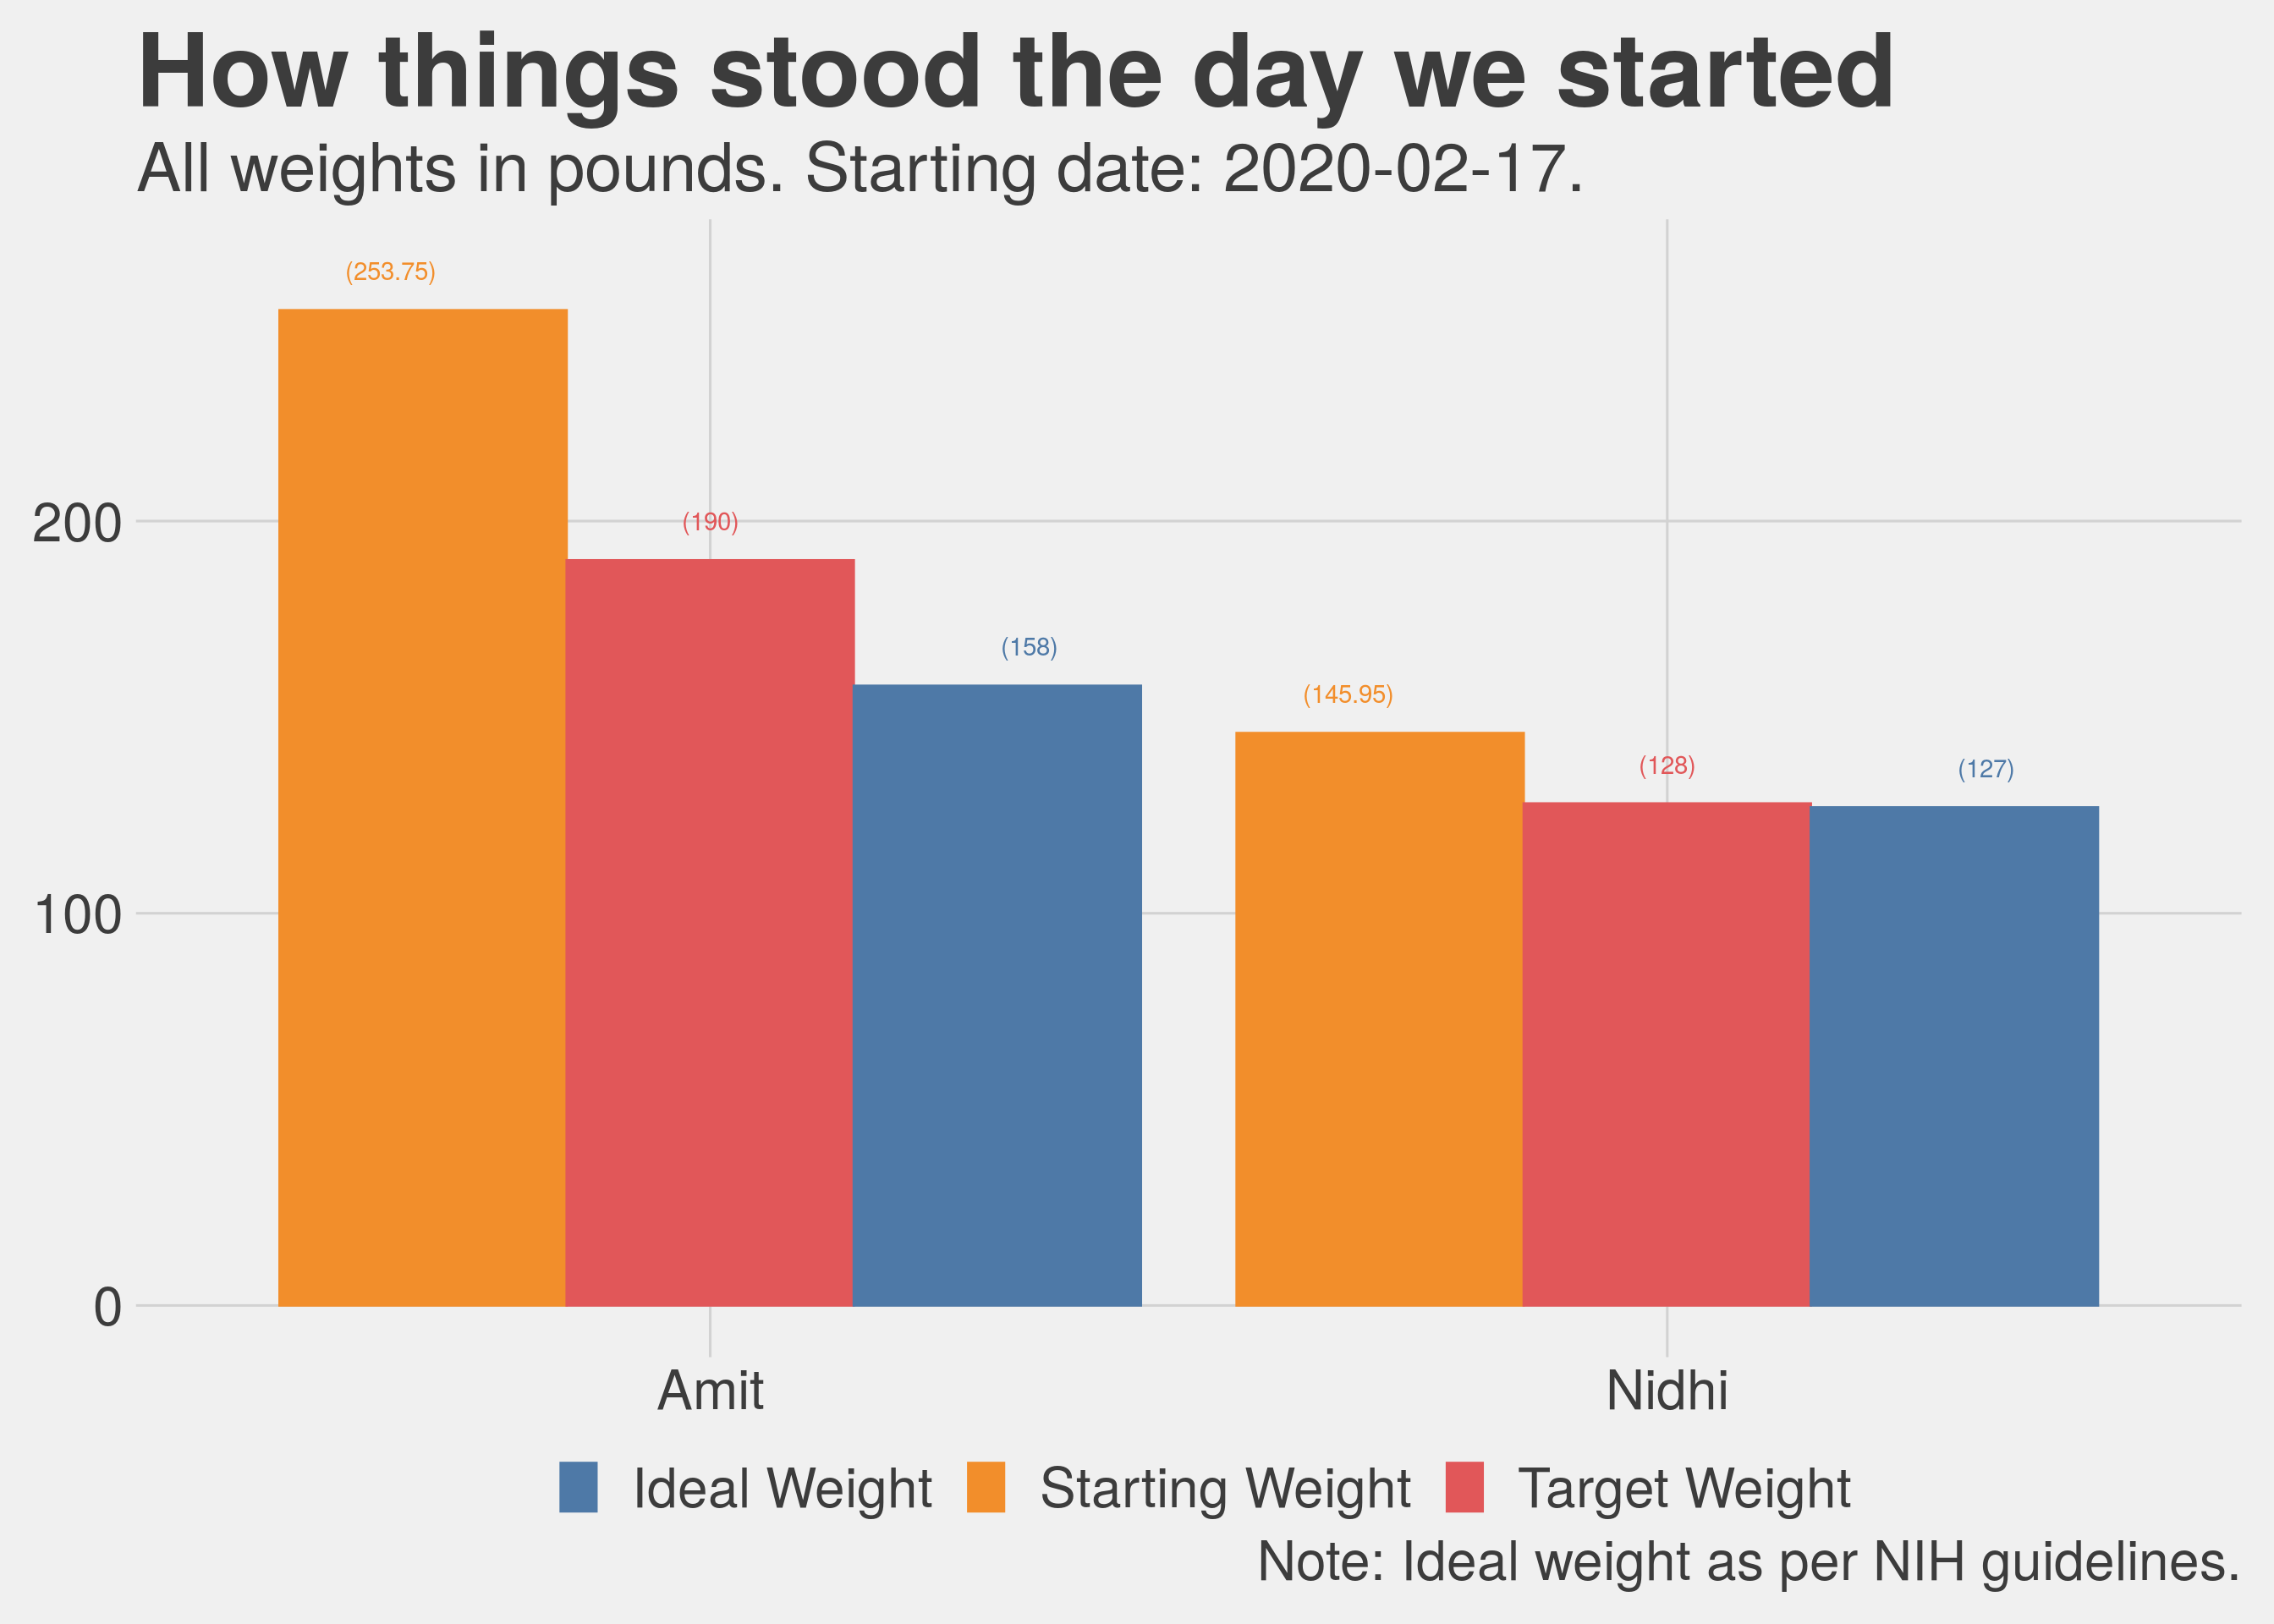
\includegraphics{bookdownproj_files/figure-latex/unnamed-chunk-4-1.pdf}

\chapter{Clean Eating}\label{clean-eating}

\emph{Disclaimer: this is my interpretation of what i understood and did
as part of clean eating. I am not aware if there is a standard
definition for this and if there is one i do not wish to challenge
whatever it is.}

Clean eating is not a diet. This is the number one thing i find myself
explaining to people when they say ``you have lost so much, what diet
are you following''. It is simply a decision of saying i am going to
keep processed foods and sugars out of my body. Strictly speaking, only
if you are eating something you have grown or you have hunted are you
eating clean, but then let's be real here, unless you are living on a
farm, this is not feasible. The next best thing we could do is to keep
processed food and especially processed sugars out of our body. I dont
need to say more on this except that there is tonnes of research
available proving why processed food and refined sugars are just plain
bad, do yourself a favor stay away from these.

Appendix A contains a checklist of what we confirmed with our trainer
was allowed during clean eating. This is pretty exhaustive list. Before
i get into the details of exactly what we ate, i would like to address
something upfront. Is clean eating hard? Yes it is hard, but only to the
extent of saying that nothing that is worthwhile is ever easy. Not being
able to eat ice-creams (substitute with your favorite unhealthy snack)
is hard, i am not going to lie, but then it is for a fixed period of
time and also, nobody ever became unhealthy because they did not eat
ice-cream. At the same time, clean eating is also not that hard when i
compare it to other diets. The key difference is that you are not
counting calories, counting calories is not sustainable, you cannot
survive on a 1000 calories a day for long (several months maybe, can you
do it for your whole life). Think of it, if counting calories was the
solution then some food company would have figured it out and the
shelves would be full of some magic food.

The intent of clean eating is to reset your system, recaliberate your
taste buds so that they begin to appreciate the natural tasts of
different foods. I would know because i am the person who back in India
would go (every now and then) for a late evening after dinner ice-cream
(a fruit salad sunday to be precise) and then as if that was not sweet
enough, go to a kulfi place right after that to top it off. 3 weeks into
clean eating i found a papaya to be sweet, grapes to be just too sweet
and eating an orange or two as a 4pm snack seemed delightful.

Indulge me a little bit before we get into the details of
breakfast/lunch/dinner. So, when we got married, we went to Europe for
our honeymoon and one of the places we visited was the cite of Nice in
south of France, absolutely beautiful place, however, we did not quite
develop an appreciation for French food, so we were looking for some
Indian food or anything that had some spices and was not cold and bland
(my apologies to anyone reading and thinking these folks don't know the
first thing about French food). We found this Pakistani restaurant by
the beach and were delighted to eat some Butter Chicken there. It was
not hard to notice that we were from India because Nidhi was still
wearing some distinctly Indian (more appropriate to say Indian
sub-continent) jewellery. The owner of the restaurant stopped by to talk
to us and seeing we were Indian sat down for a conversation. He said,
``you know, the French food is the best food in the world'', we were
listening but not quite agreeing, the butter chicken would not allow me
to agree, he continued ``back home, we put so much spices in our food,
cook it for so long that we never get to know what the ingredients
actually tasted like\ldots{}''. Months of eating relatively clean (not
strictly, i mean i do eat my ice-cream sometimes, i have had a pizza
once or twice in the last 6 months), have made me realize that while i
still cannot compare the taste of the Indian cooking with anything else,
i do see the point of the natural taste of food. Our elder son likes a
green chilly with his dinner, but the younger one does not recognize
that ``bitter'' can also be a taste.

\section{A clean breakfast}\label{a-clean-breakfast}

Breakfast was mostly eggs, in every form. Egg fry (use Ghee or kerrygold
butter), omlette (sometimes with tiny pieces of bacon thrown in), boiled
eggs, scrambled eggs or any other variation you can think of. Along with
coffee (for me, i am a coffee person) or tea (Nidhi is a tea person)
with almond milk or an almond and coconut milk creamer. We do not eat
eggs or meat on Tuesdays, so the eggs were replaced with bananas or
almond flour pan cakes. Another thing we really enjoyed for breakfast
was frozen Acai bowl (you can get them at Costco, just don't eat the
granola that comes along with it).

Here are some pictures. I would note that everyday the omlette may not
have looked as good but was pretty close. It is real hard work to make
breakfast this good everyday and the credit for this is one person's and
one person's alone i.e.~Nidhi :).

\begin{figure}
\centering
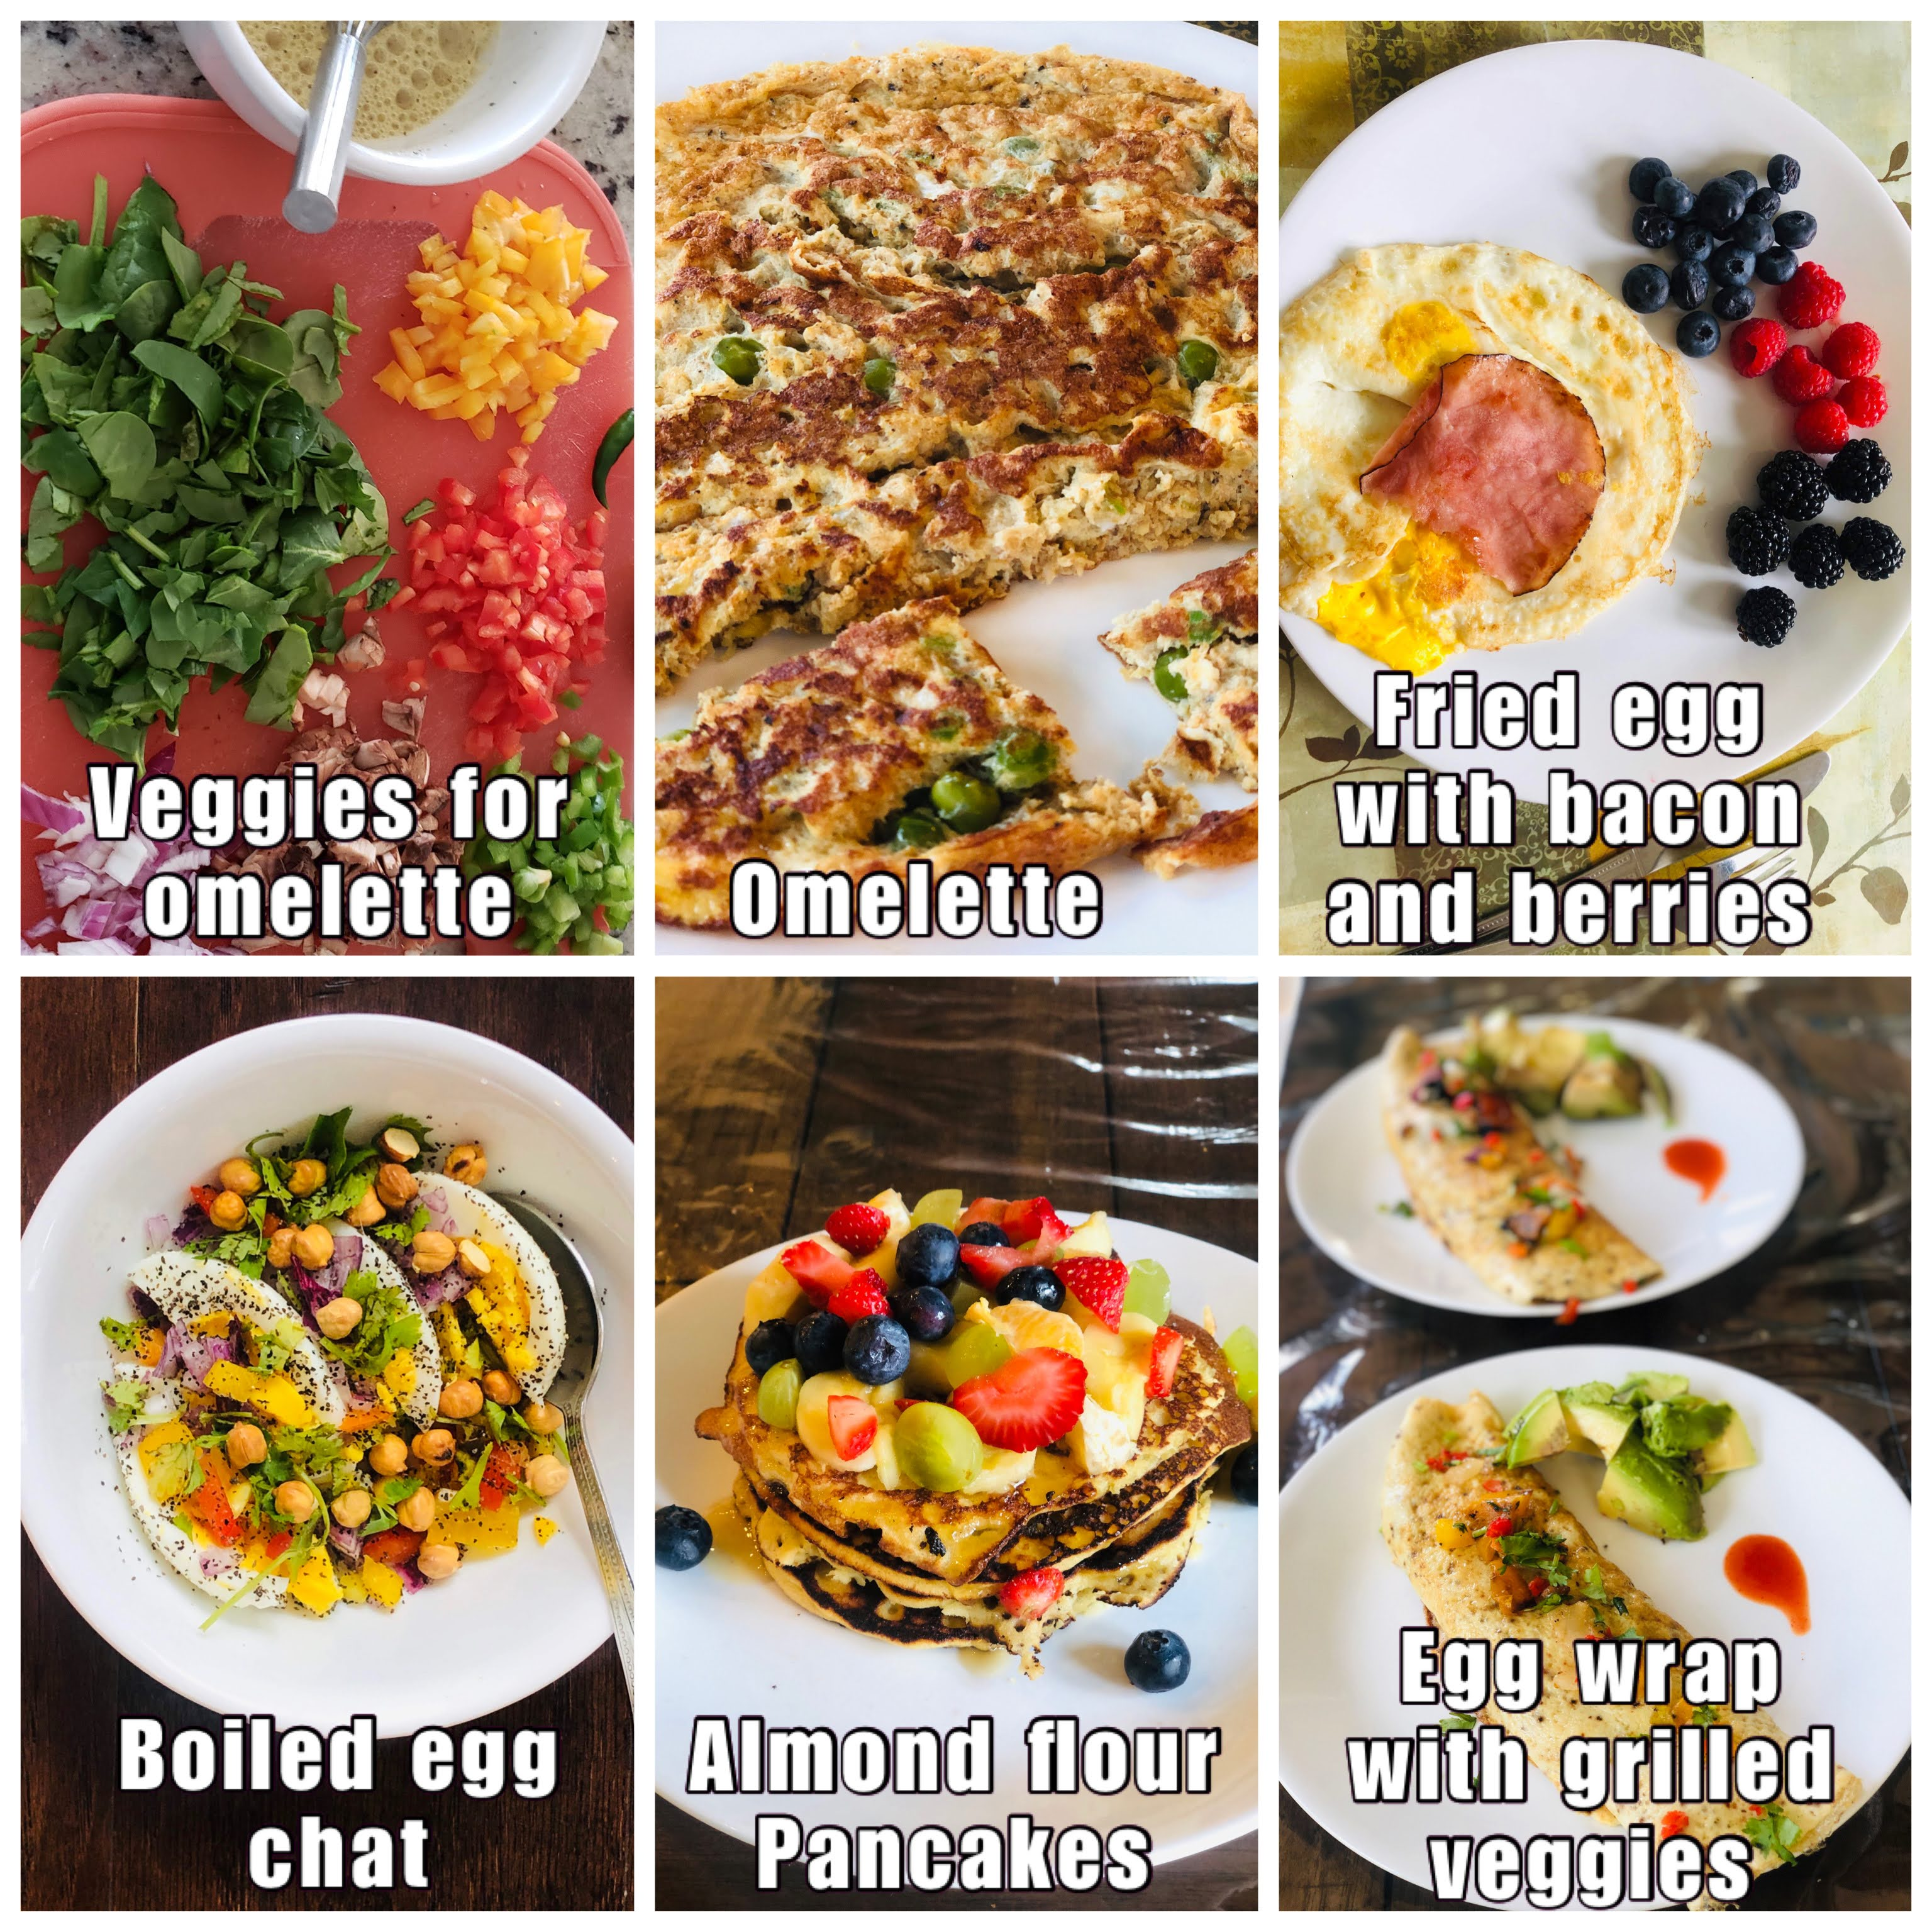
\includegraphics{pictures/breakfast.JPG}
\caption{A clean breakfast}
\end{figure}

\section{A lunch we really love}\label{a-lunch-we-really-love}

For lunch we used to have salads. I don't know about you but when i
think of salads, i have two contrasting pictures in my head as reference
(this is all prior to clean eating), one is a cold salad with raw
vegetables and boiled eggs, along with some beans and chickpeas, maybe
mushrooms as well and the other image is from a salad place like the one
i visited often at Georgetown university, exquisite salads with all
sorts of ``woke'' ingredients. The first one was something i just did
not find palatable at all and the second one was what i would wait for
the whole week so that i could eat it whenever i was at Georgetown for a
class. Surely there was some middle ground here, i would think, and
there is.

Costco has a bunch of good salad mixtures in their frozen section and
they are all very good. We particularly liked the sweet kale salad. So
we mixed the sweet kale, with additional ingredients such as spinach or
other mixed greens and topped it with sunflower seeds, chia seeds,
walnuts (sometimes cashews), some cranberries and my favorite,
``blueberries''. Used a home made dressing made of olive oil and TBD
ingredients. Add a boiled egg, half an avocado and then either some
grilled chicken or tuna. For Tuesdays' we substituted chicken/tuna with
grilled tofu. Congratulations! you have just made yourself an awesome
salad. I am still surprised then even after more than 6 months of eating
variants of it (keeping the base receipe the same) 4 to 5 times a week,
we are still not bored of it, in fact we seem to like it as much as we
liked it before.

\begin{figure}
\centering
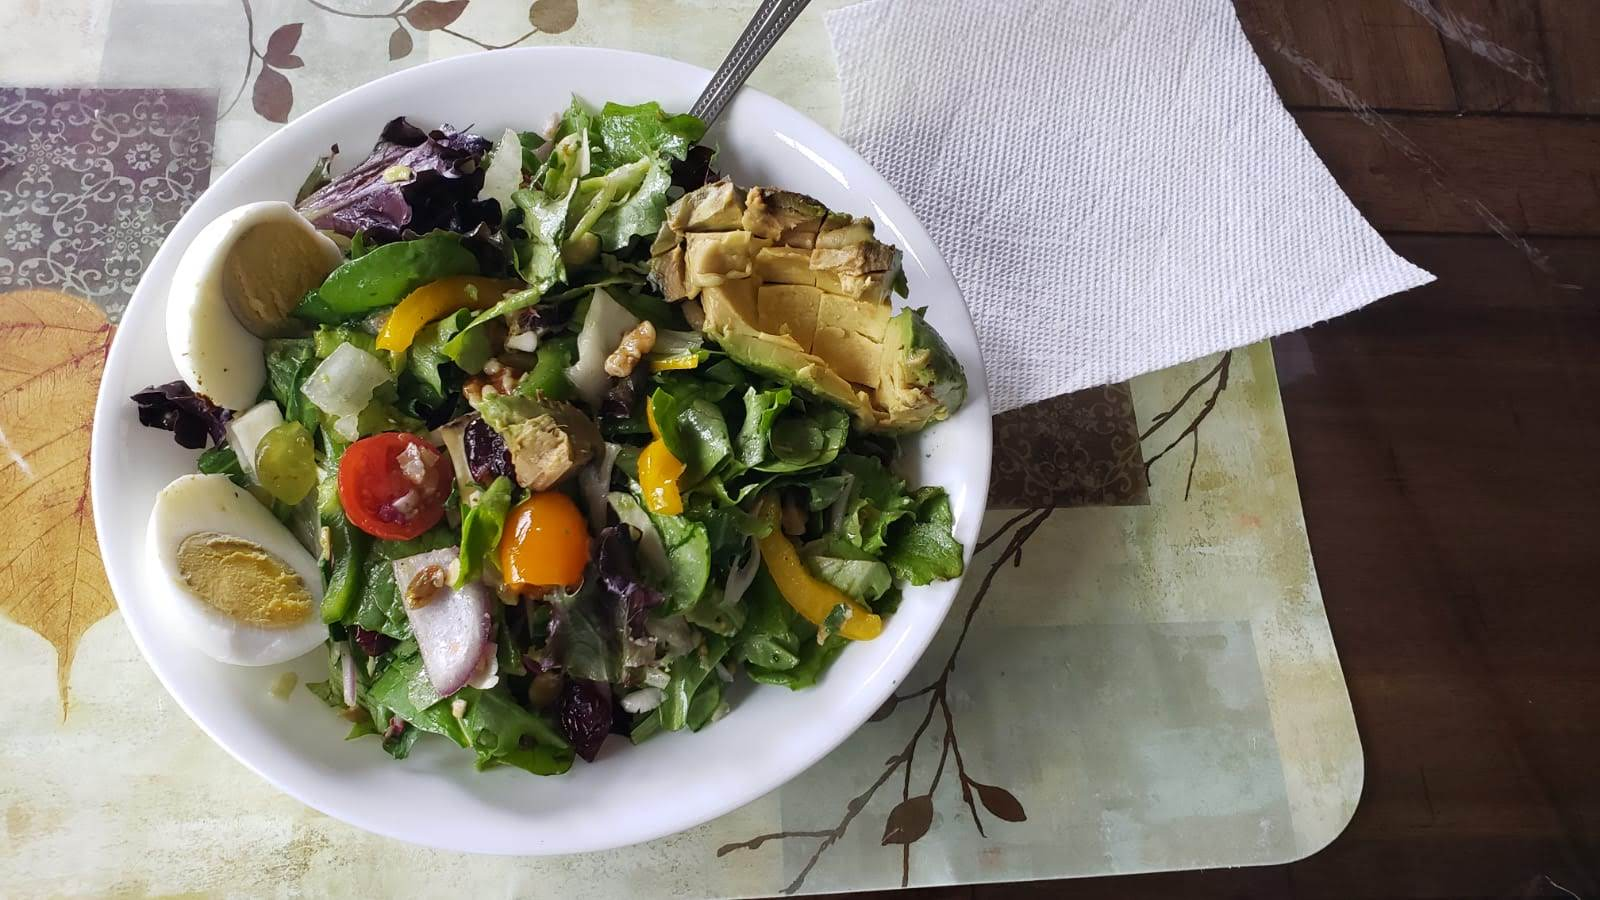
\includegraphics{pictures/everyday-salad.jpg}
\caption{The everyday salad}
\end{figure}

\begin{figure}
\centering
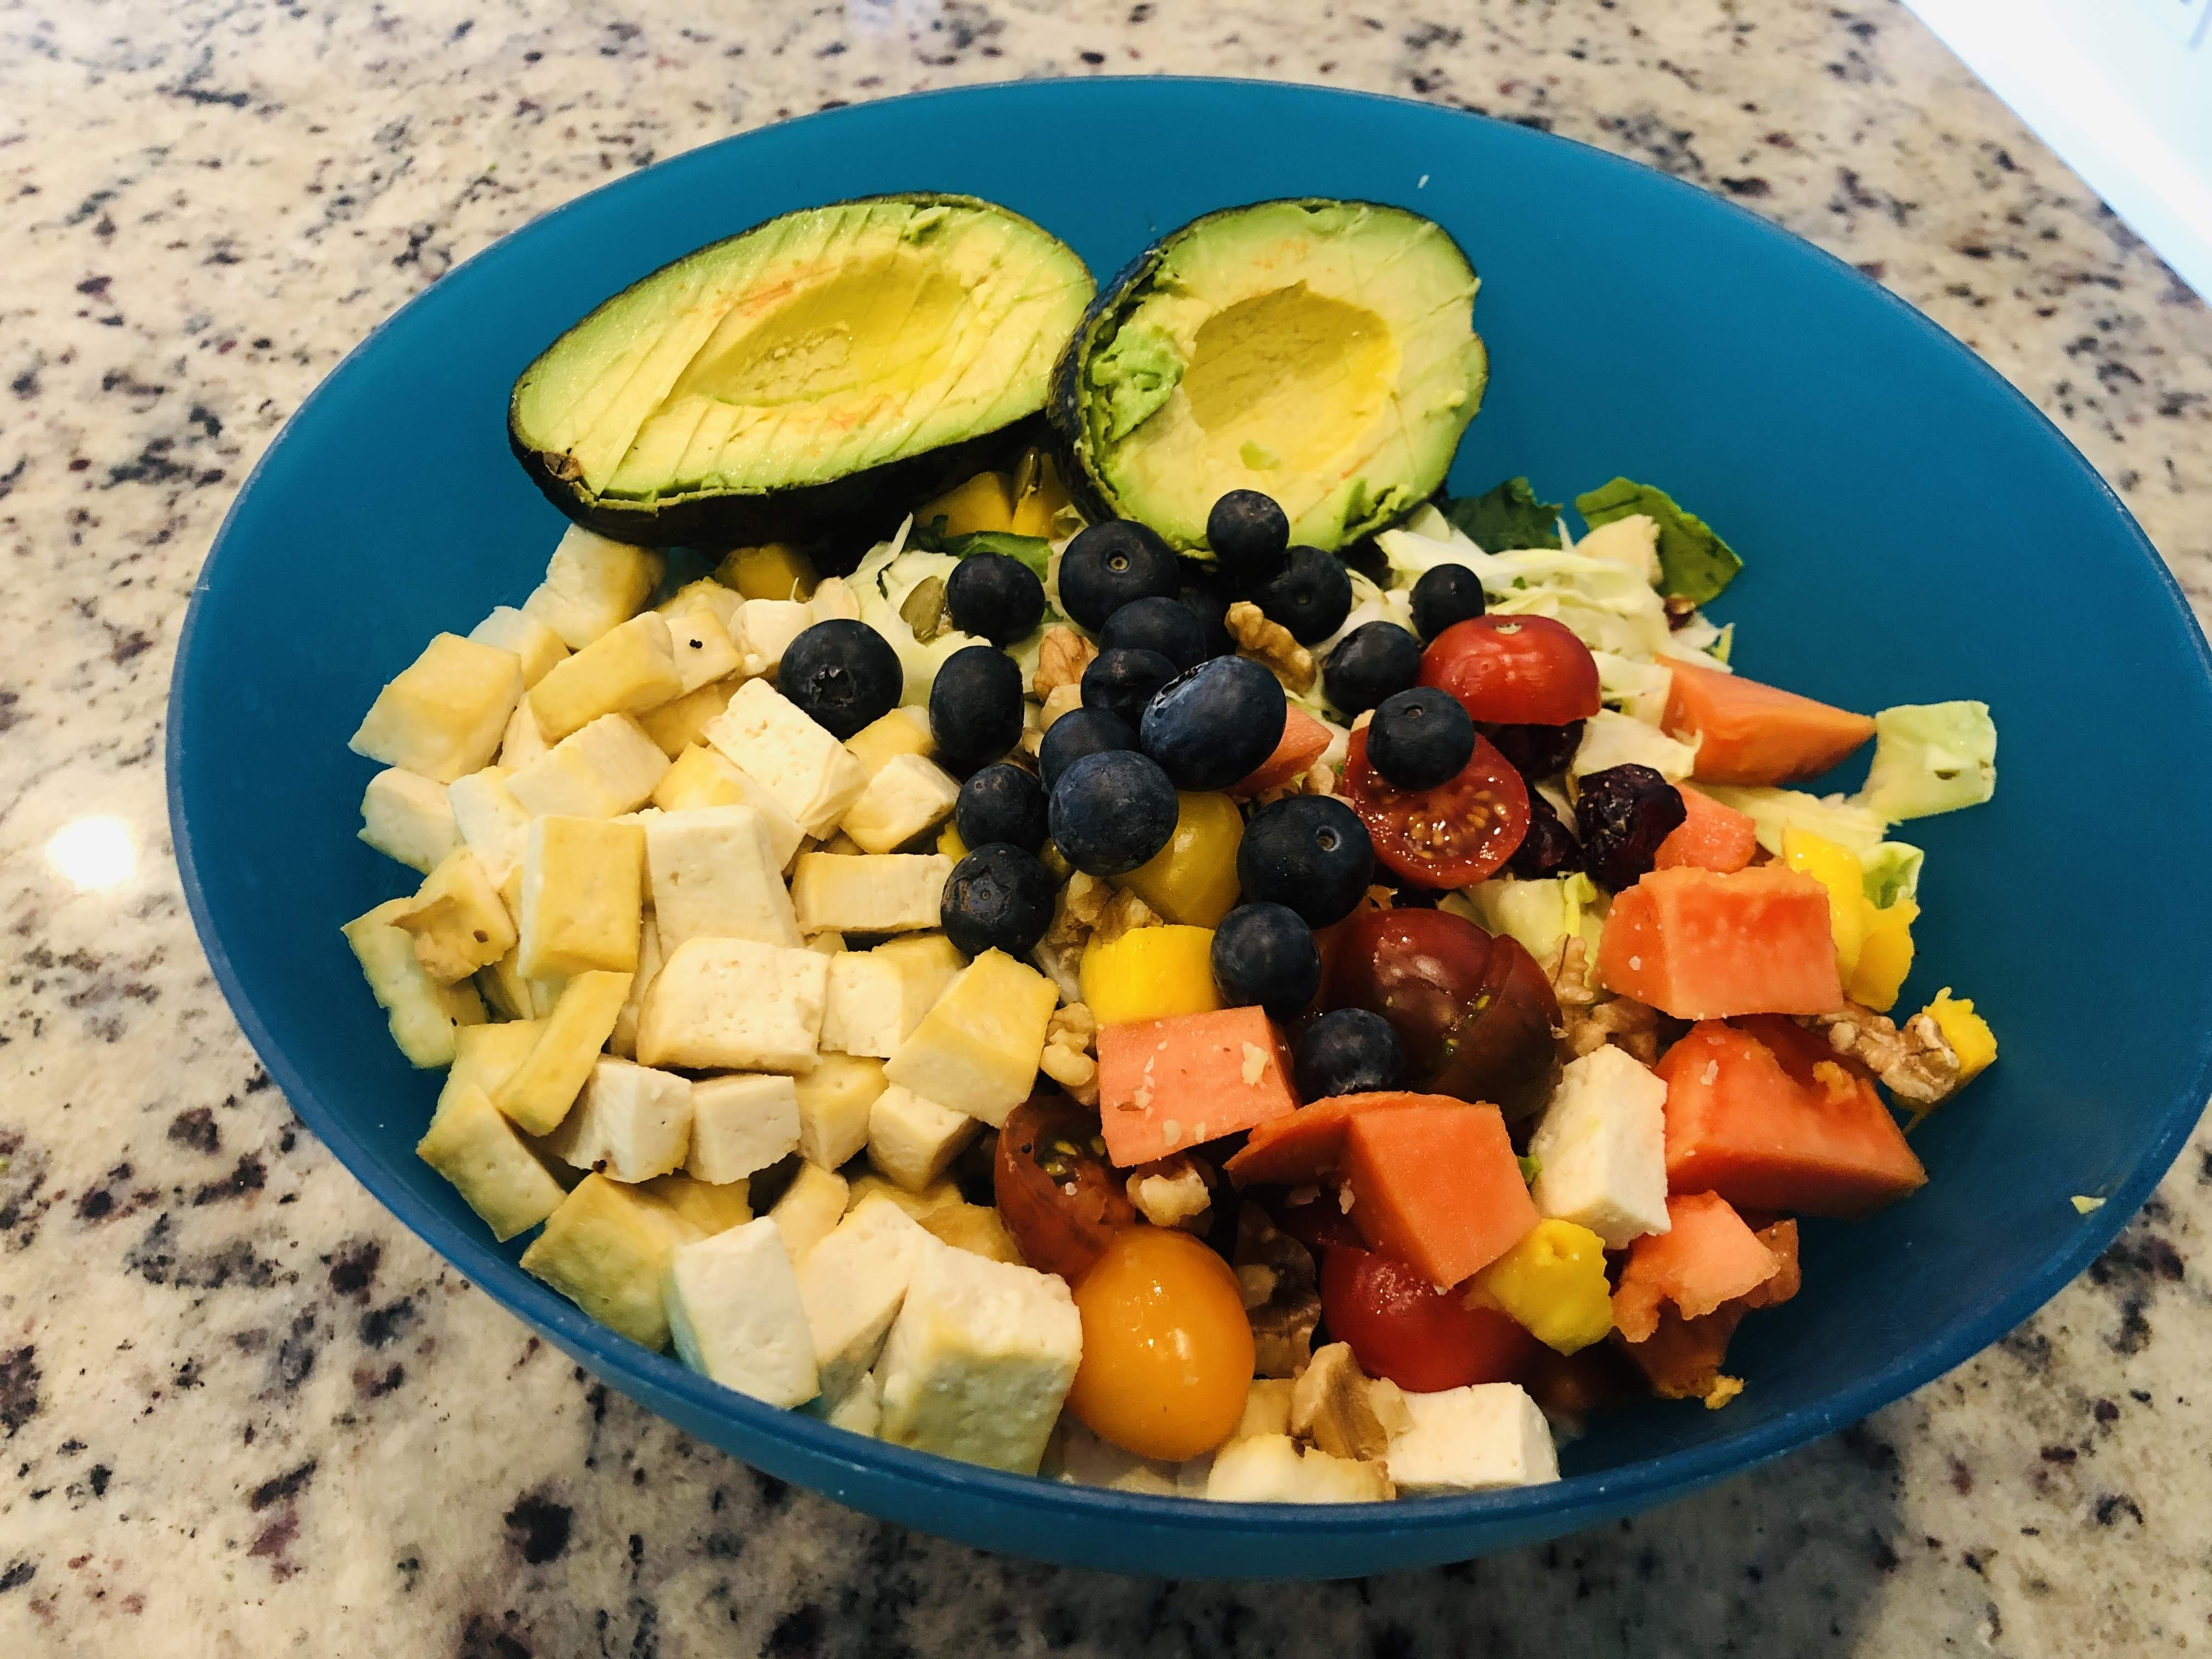
\includegraphics{pictures/the-tuesday-salad.jpg}
\caption{The Tuesday salad}
\end{figure}

\begin{figure}
\centering
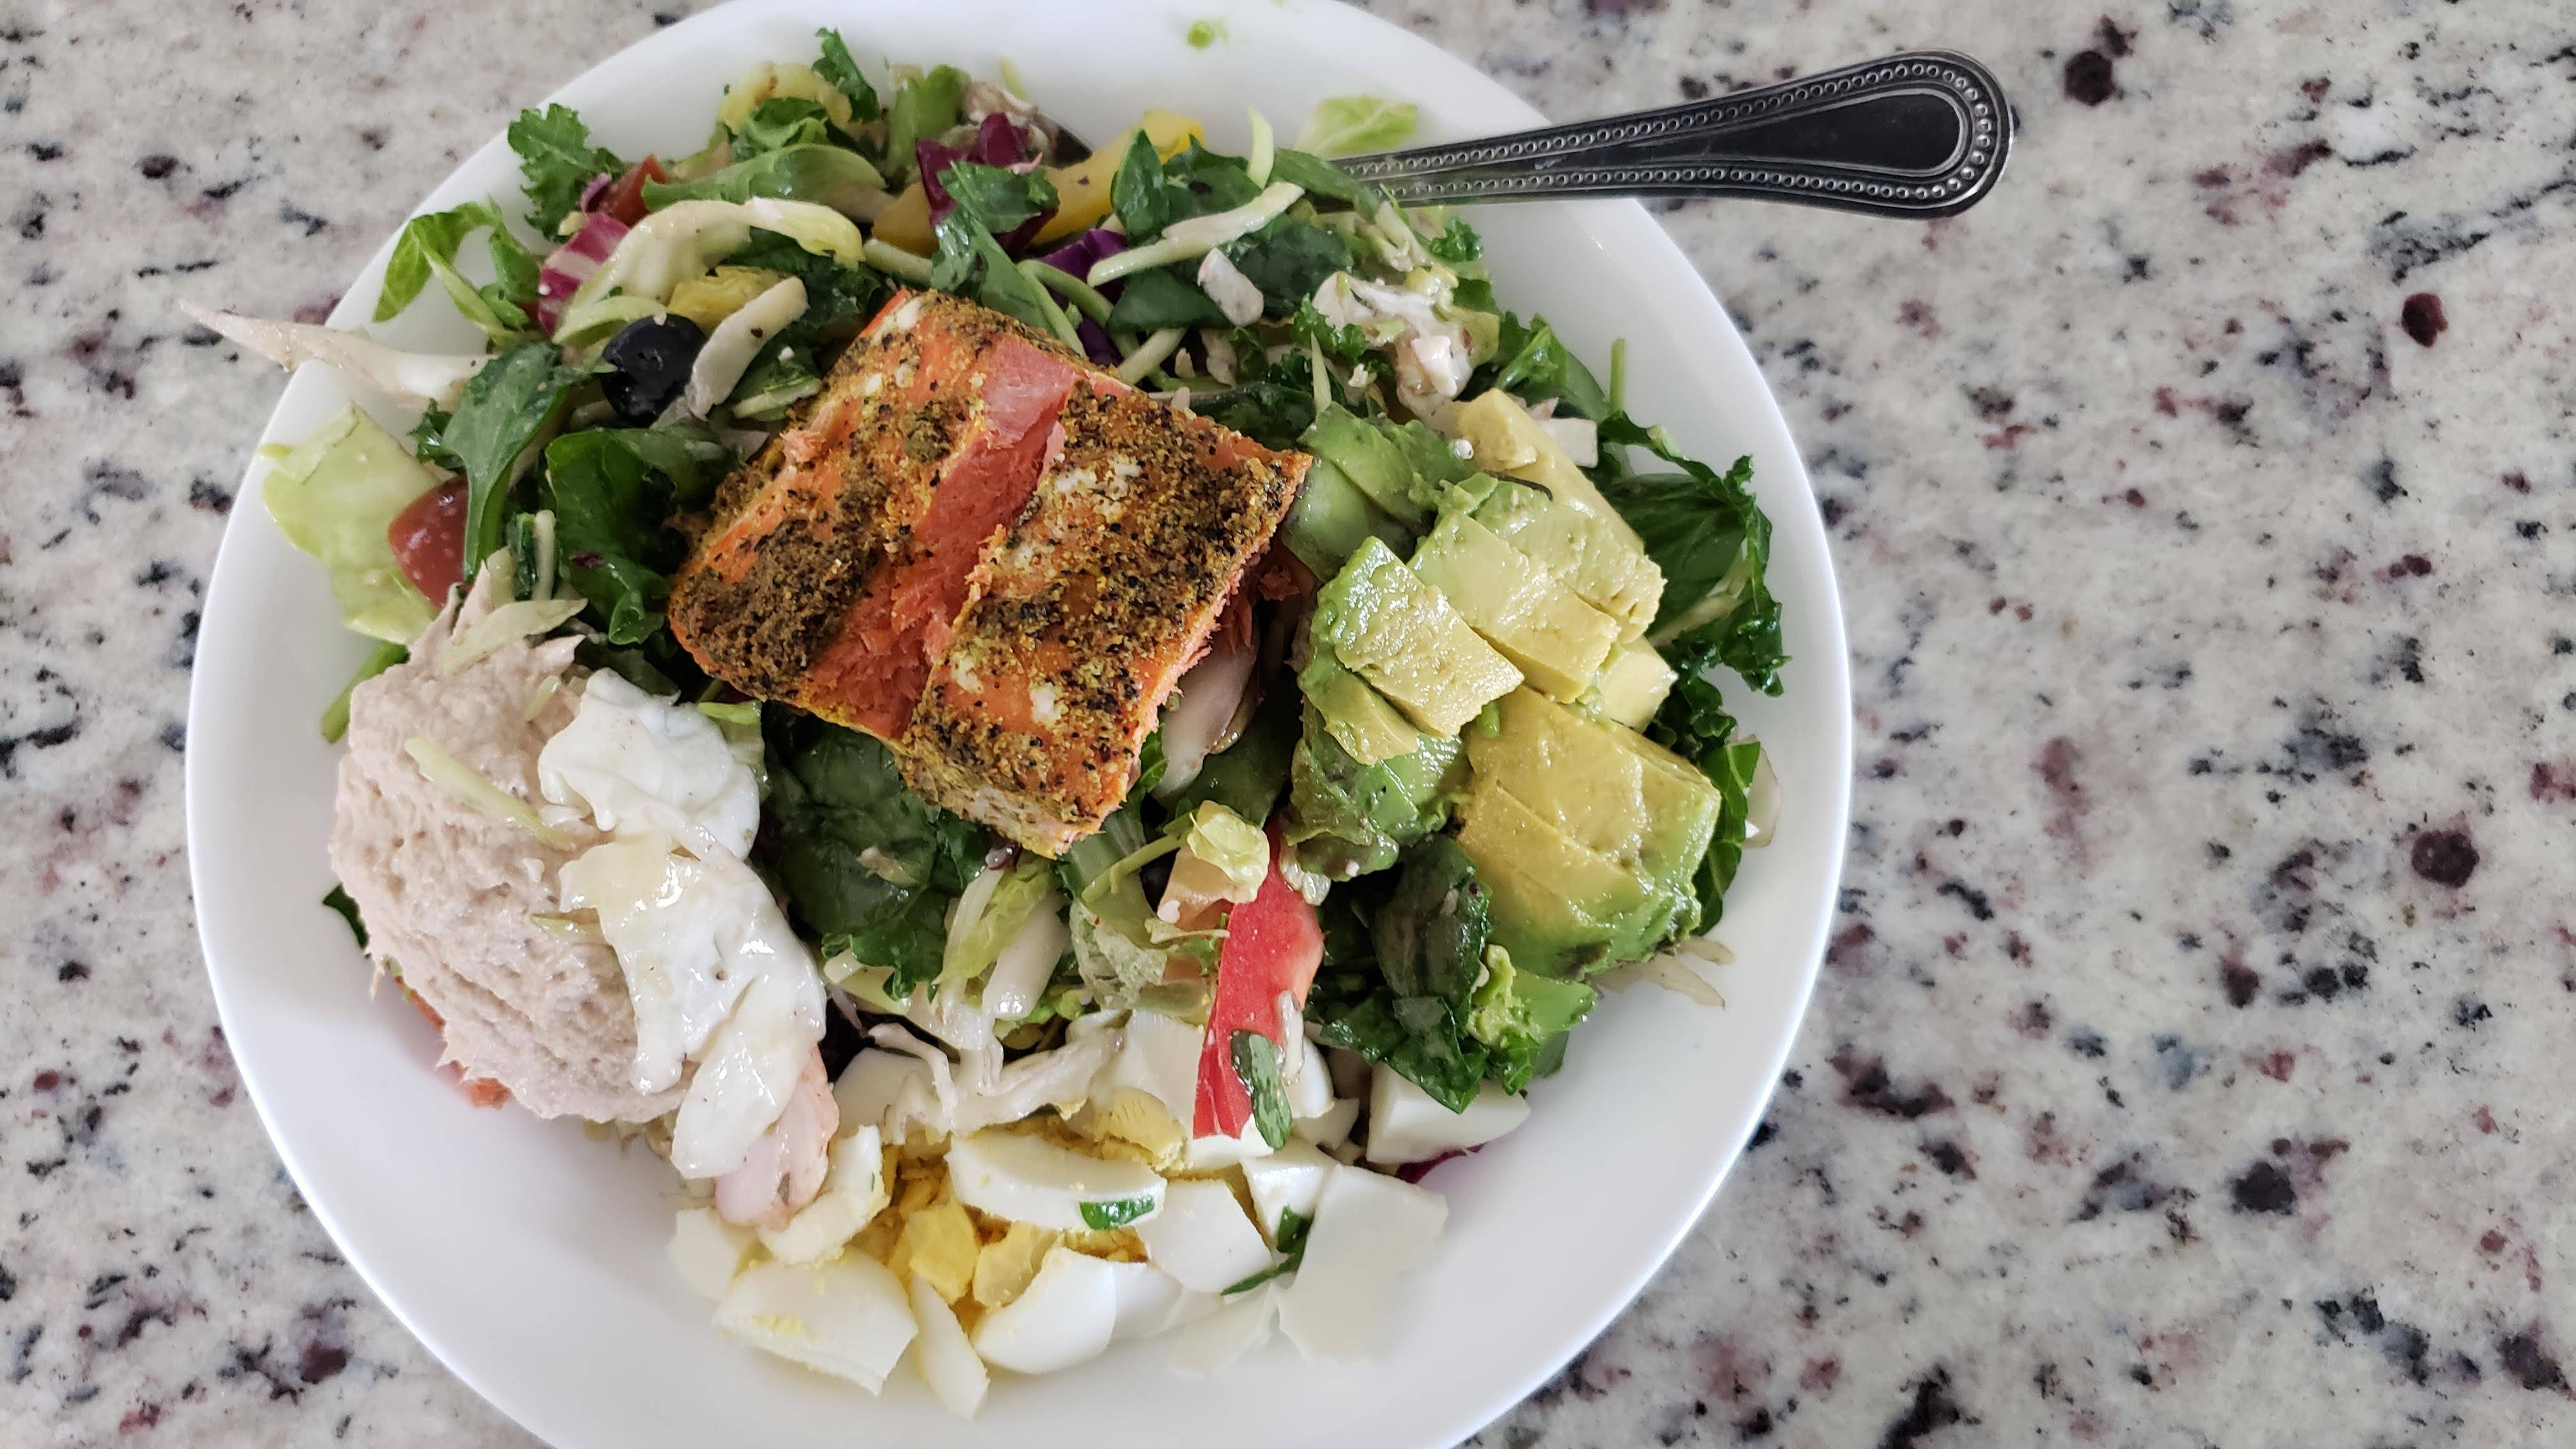
\includegraphics{pictures/tuna-treat-salad-w-salmon-for-company.jpg}
\caption{The awesome tuna and salamon salad}
\end{figure}

\begin{figure}
\centering
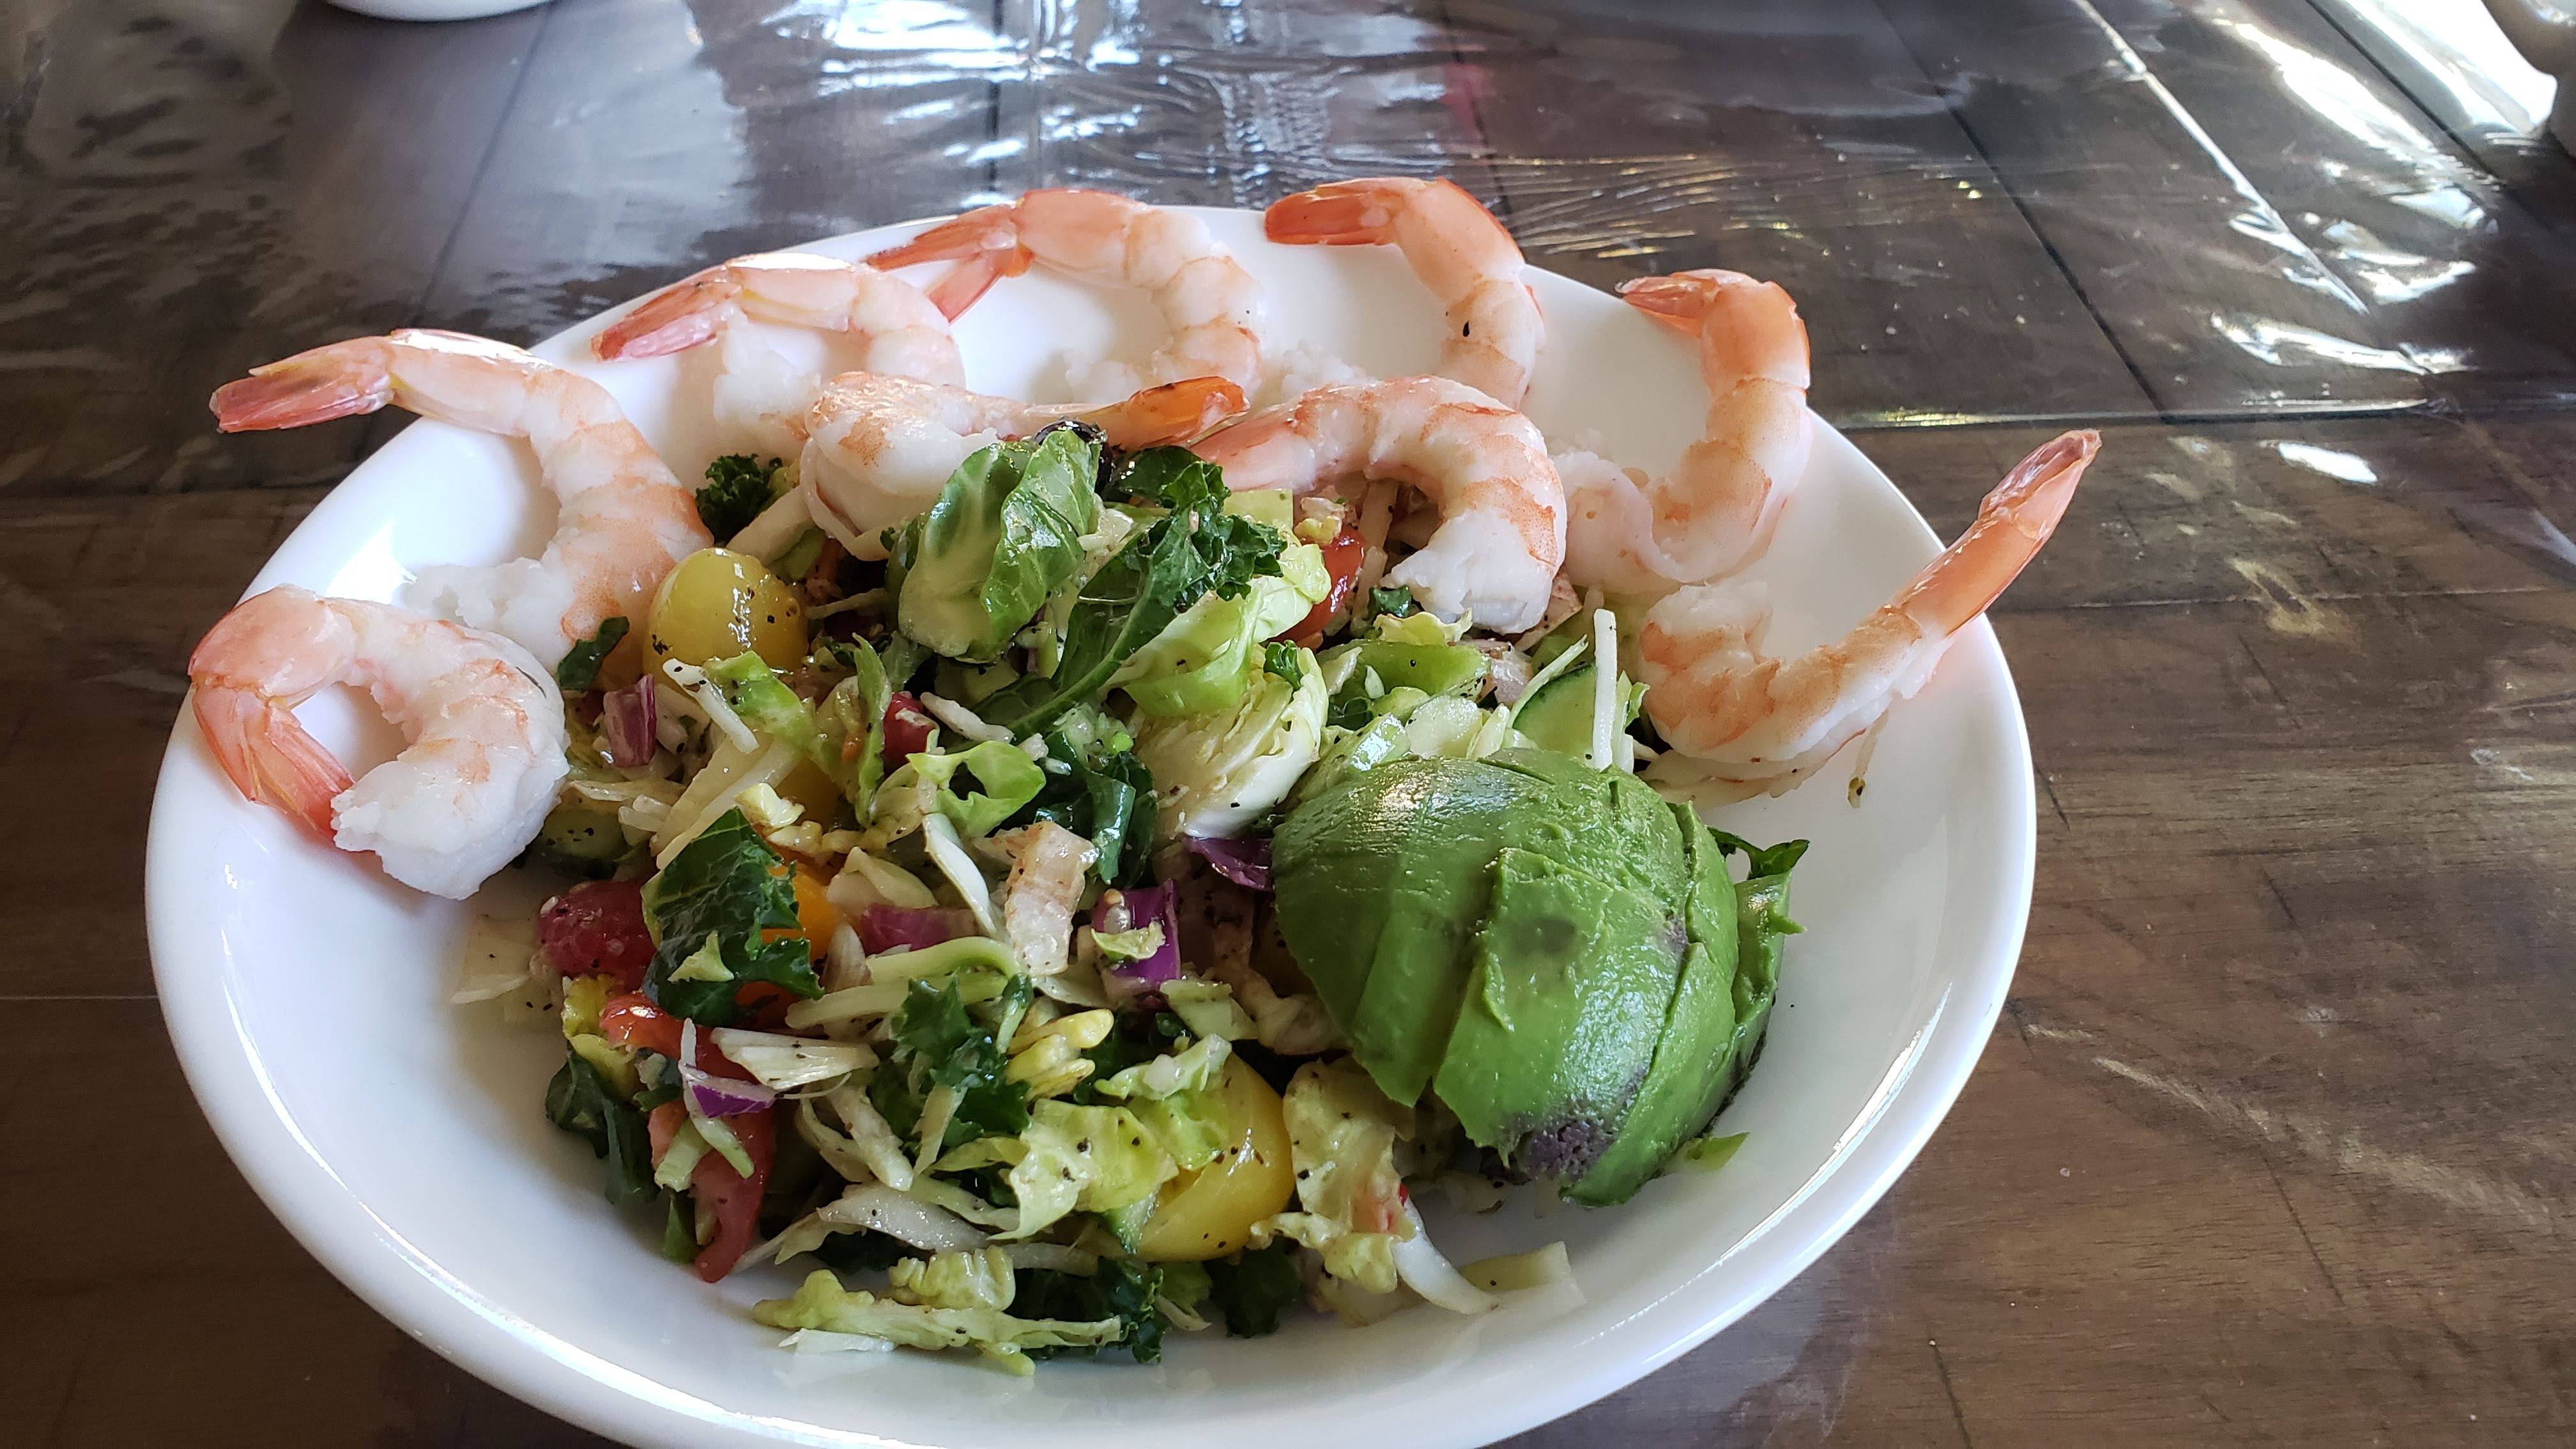
\includegraphics{pictures/shrimp-salad.jpg}
\caption{The I want to eat something special shrimp salad}
\end{figure}

One of thoughts i had and i believe many people would have is that salad
does not satiate me, it does not full me up. That is actually not true,
or was not certainly true for me as i found out. Eating a bowl and a
half of salad does indeed fill you up. The test for me was that after my
lunch i usually liked to drink hot coffee just to, you know, wash it
down, and that need did not go away after switching to salads for lunch.
I still like a cup of hot coffee after lunch. What does happen is that
after 2 to 3 hours i felt the need for a mid afternoon snack. Previously
this could have been any unhealth options like chips, cookies, a diet
soda, even a snickers bar, basically anything you would typically find
in a vending machine. That had to go, and it did.

\section{The 4pm snack}\label{the-4pm-snack}

A couple of small oranges at 4pm felt delightful. They tasted good, and
the sugar content provides the boost the brain needs to shake off any
mid afternoon lethargy or drowsiness. At times i also ate maybe 4 to 5
apricots, maybe an apple, or even some nuts such as walnuts/cashew
nuts/almonds (not those packaged snack pouches please, we want to stay
away from any processed food, as much as possible).

I did not try this as much, but sometimes i did had a ``tea'' such as a
earl gray or english breakfast, just a dip tea with hot water, no milk
of any kind. It was nice, but me not being a tea person did not pursue
it that much but it is certainly an option.

\section{The grand finale a.k.a the
dinner}\label{the-grand-finale-a.k.a-the-dinner}

If you try to stick to this routine, you would naturally find that you
want to have your dinner early. What is early? For me, growing up,
dinner was never before 7.30pm and then later in life as i got caught up
with studies and then later at work and other things, it could be at 8
or 9pm or even later. That is not good, in fact, i would now say that is
just absolutely unacceptable.

Now we really make an effort to wrap up dinner by 7.30pm, maybe 8pm at
the latest. I start feeling hungry around 6pm, so a dinner around 7pm
seems like the perfect fit. Eating dinner early helps to naturally avoid
the urge for mindless snacking. As one of the people i happen to meet
over the years who was into eating healthy said ``you are not a goat,
you dont have to keep munching all the time!''. One way to avoid
munching all the time is to eat at fixed times and eat full meals so
that you dont feel hungry anymore. Instead of trying to eat just a
little bit and continue what you are doing (whether it is work or
anything else around the house) and wait for dinner, which inevitably
leads to repeated snacking while waiting for the full meal, it is much
easier to just tell your brain, wait for the full meal and then make
sure you don't push off that meal to 2 hours later.

So, what did we have for dinner, lots of different types of food and i
would happily say lots of tasty food. There is a lot of grilled food as
you would notice. I did not realize this until i wrote this, a lot of
our dinner is grilled either outside or in the oven. There are
vegetarian options also in this and let me say it for the record the
vegetarian options were as tasty as the meats.

\begin{figure}
\centering
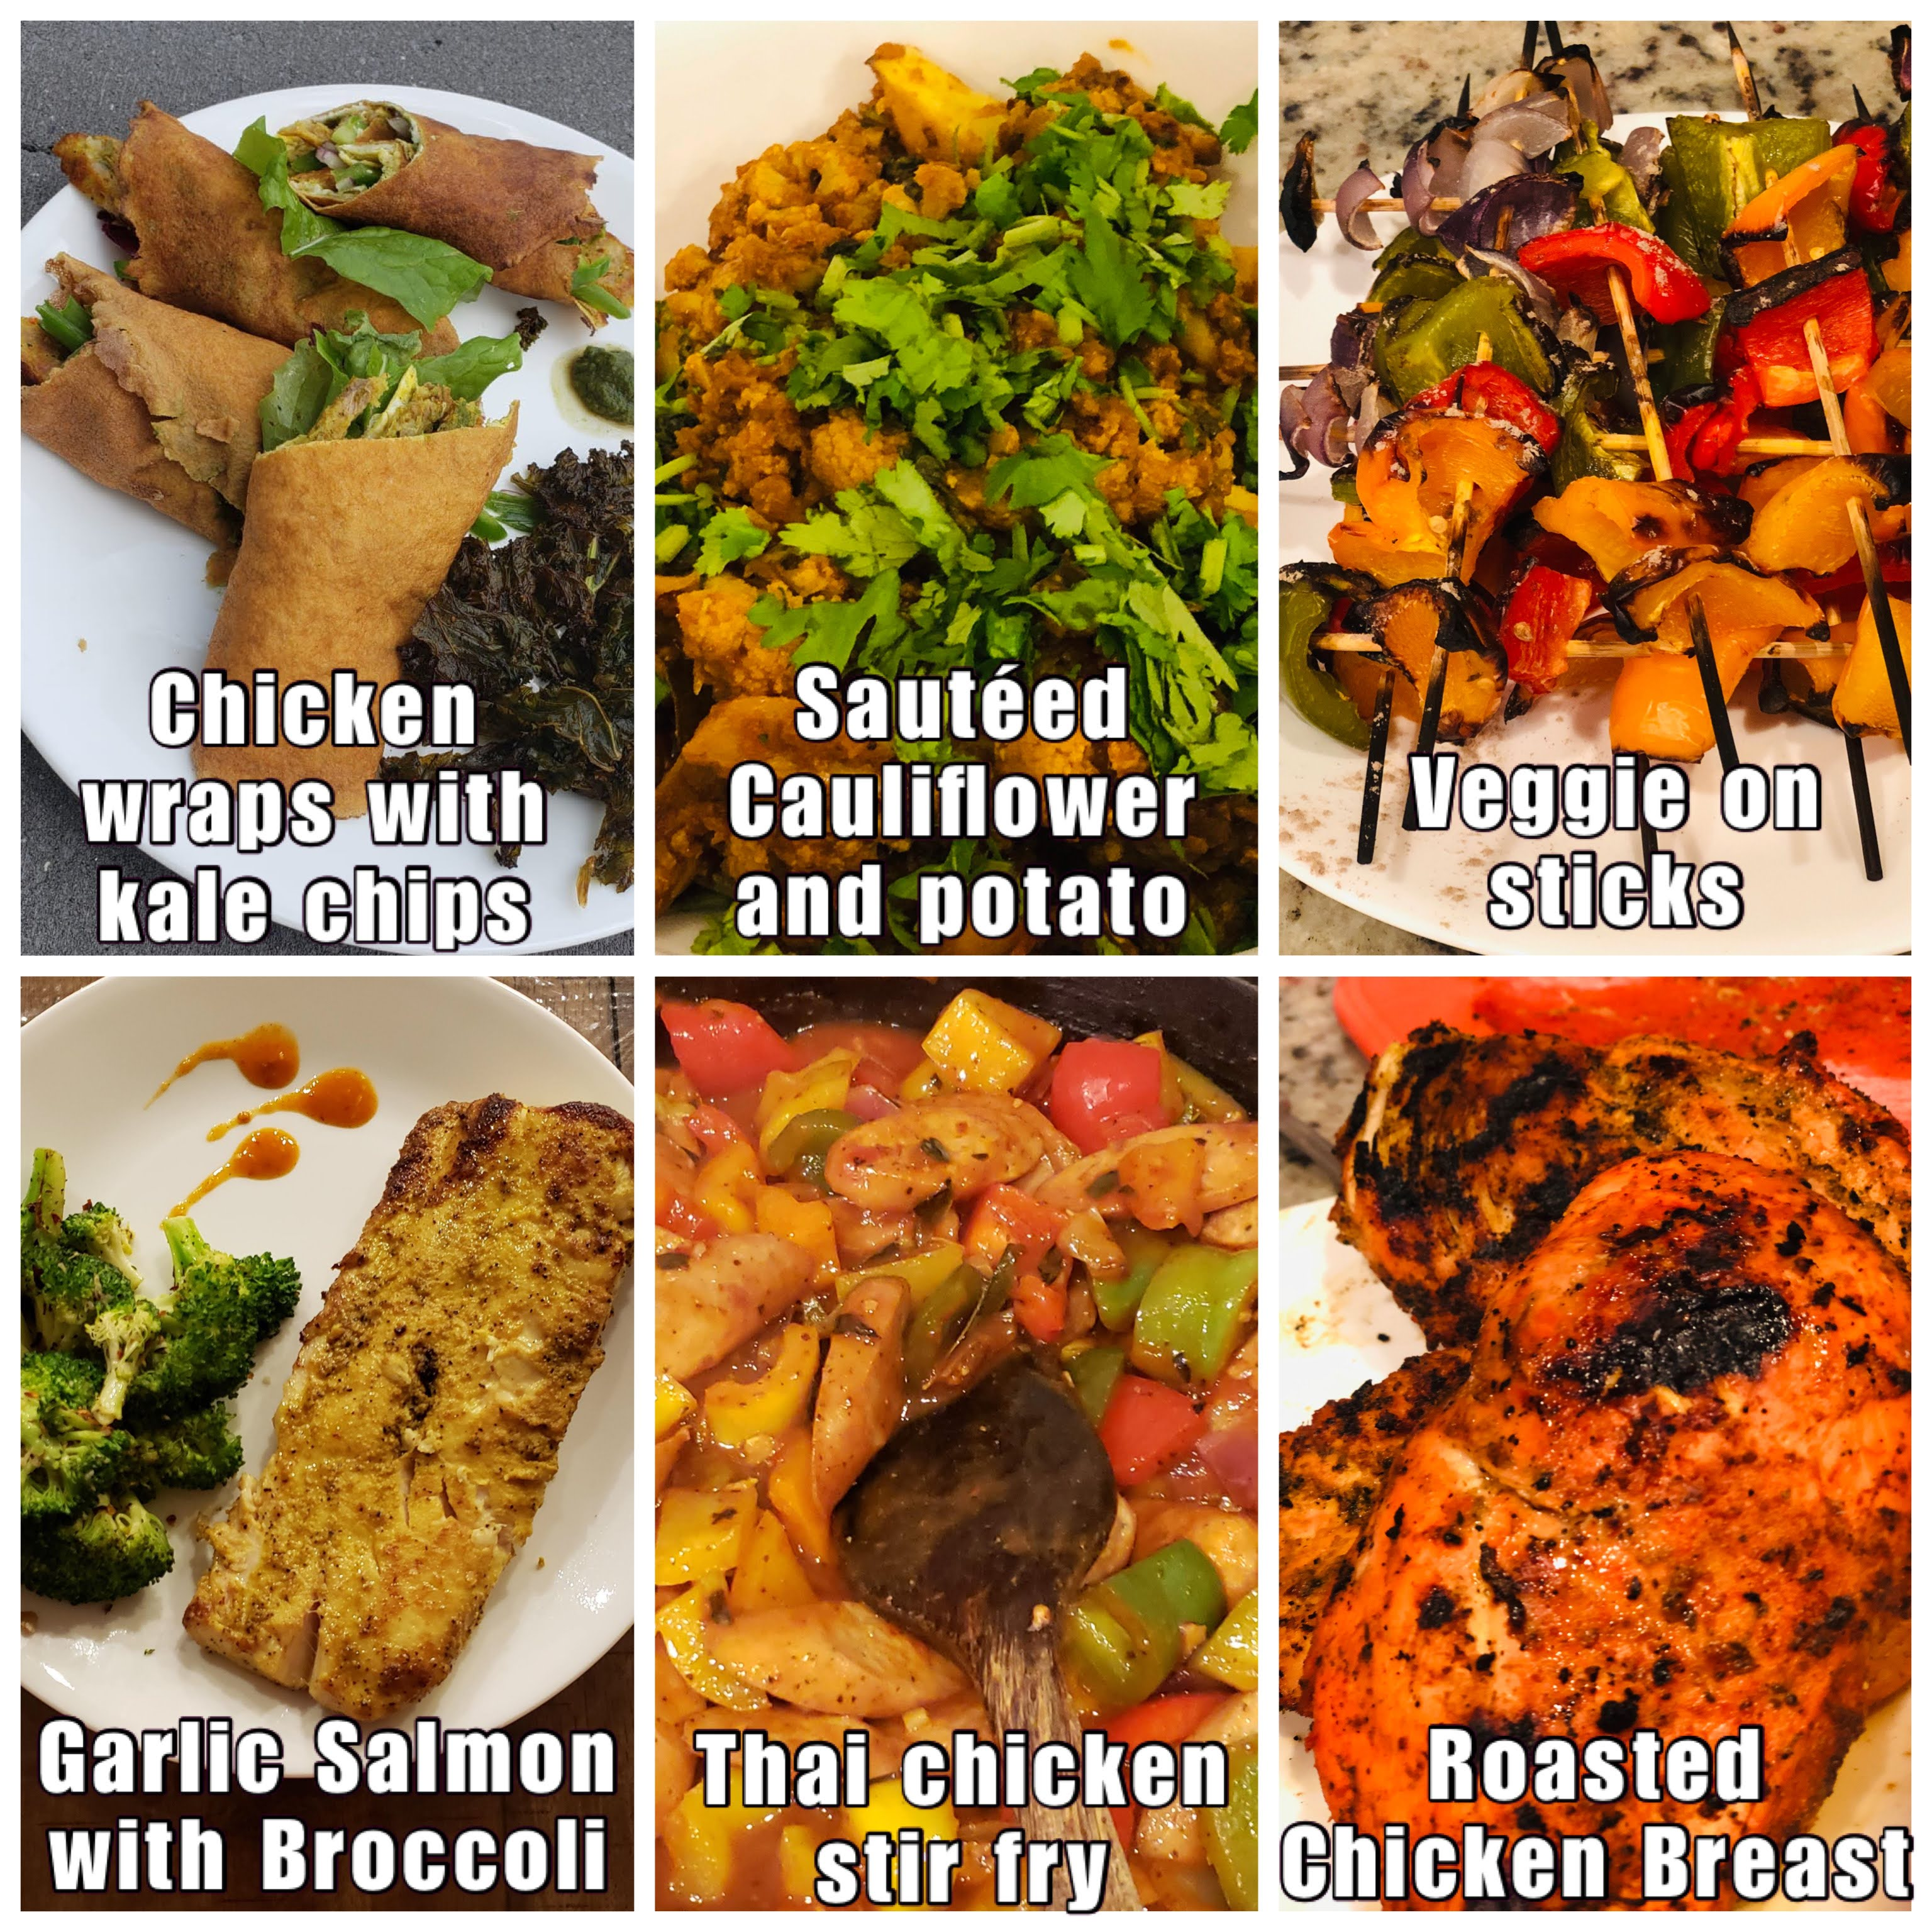
\includegraphics{pictures/dinner1.JPG}
\caption{A clean dinner}
\end{figure}

\begin{figure}
\centering
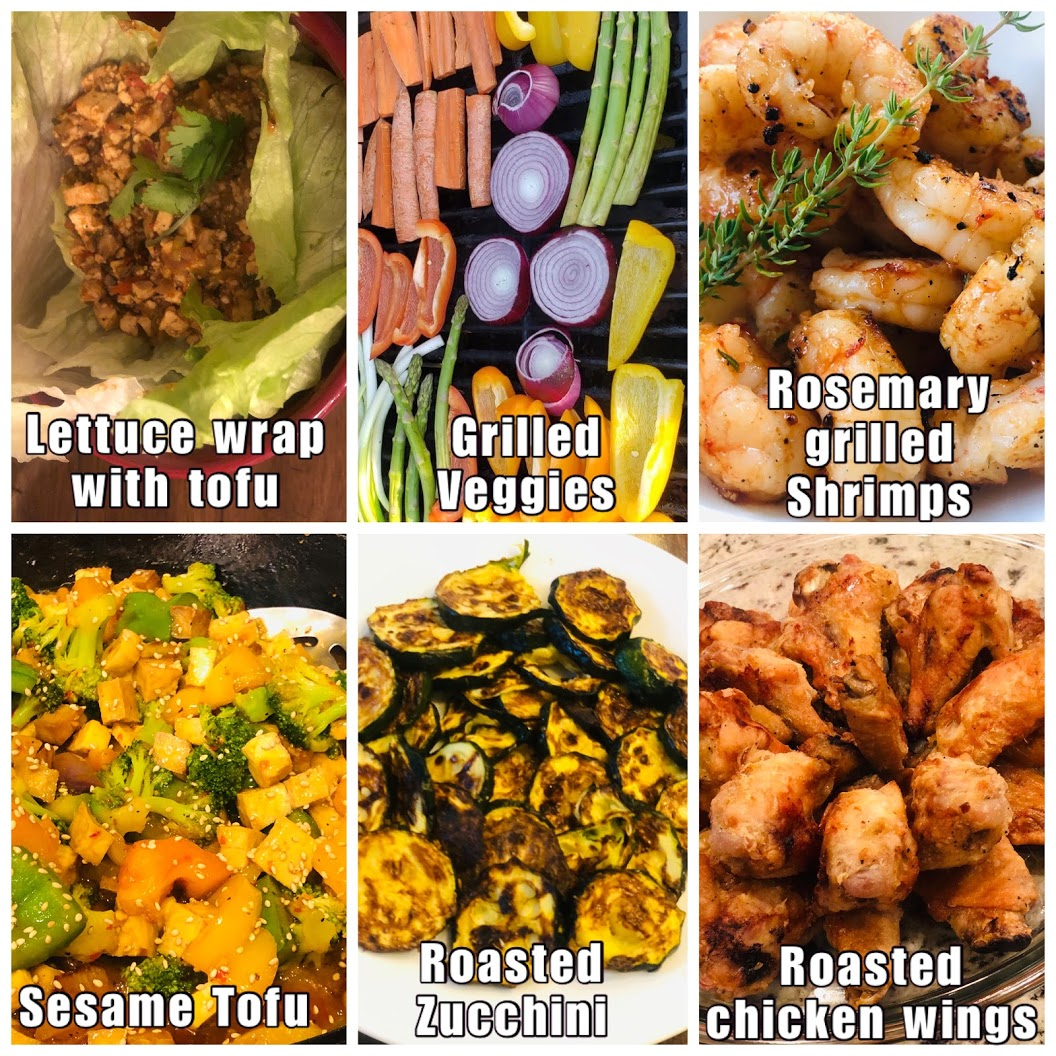
\includegraphics{pictures/dinner2.JPG}
\caption{More clean dinner}
\end{figure}

\section{The results}\label{the-results}

The following charts show our progress in terms of weight loss, with the
clean eating periods highlighted. We did a clean eating in
February-March and then another in July-August.

We saw very good results in both the iterations. The first iteration
produced much better results because obviously there was just too much
weight to lose, but surprisingly the second iteration was also very
effective. The way we see this now is that if we ever hit a really long
plateau in the journey to achieve the desired weight we could just
toughen our minds and do this again. It cannot hurt.

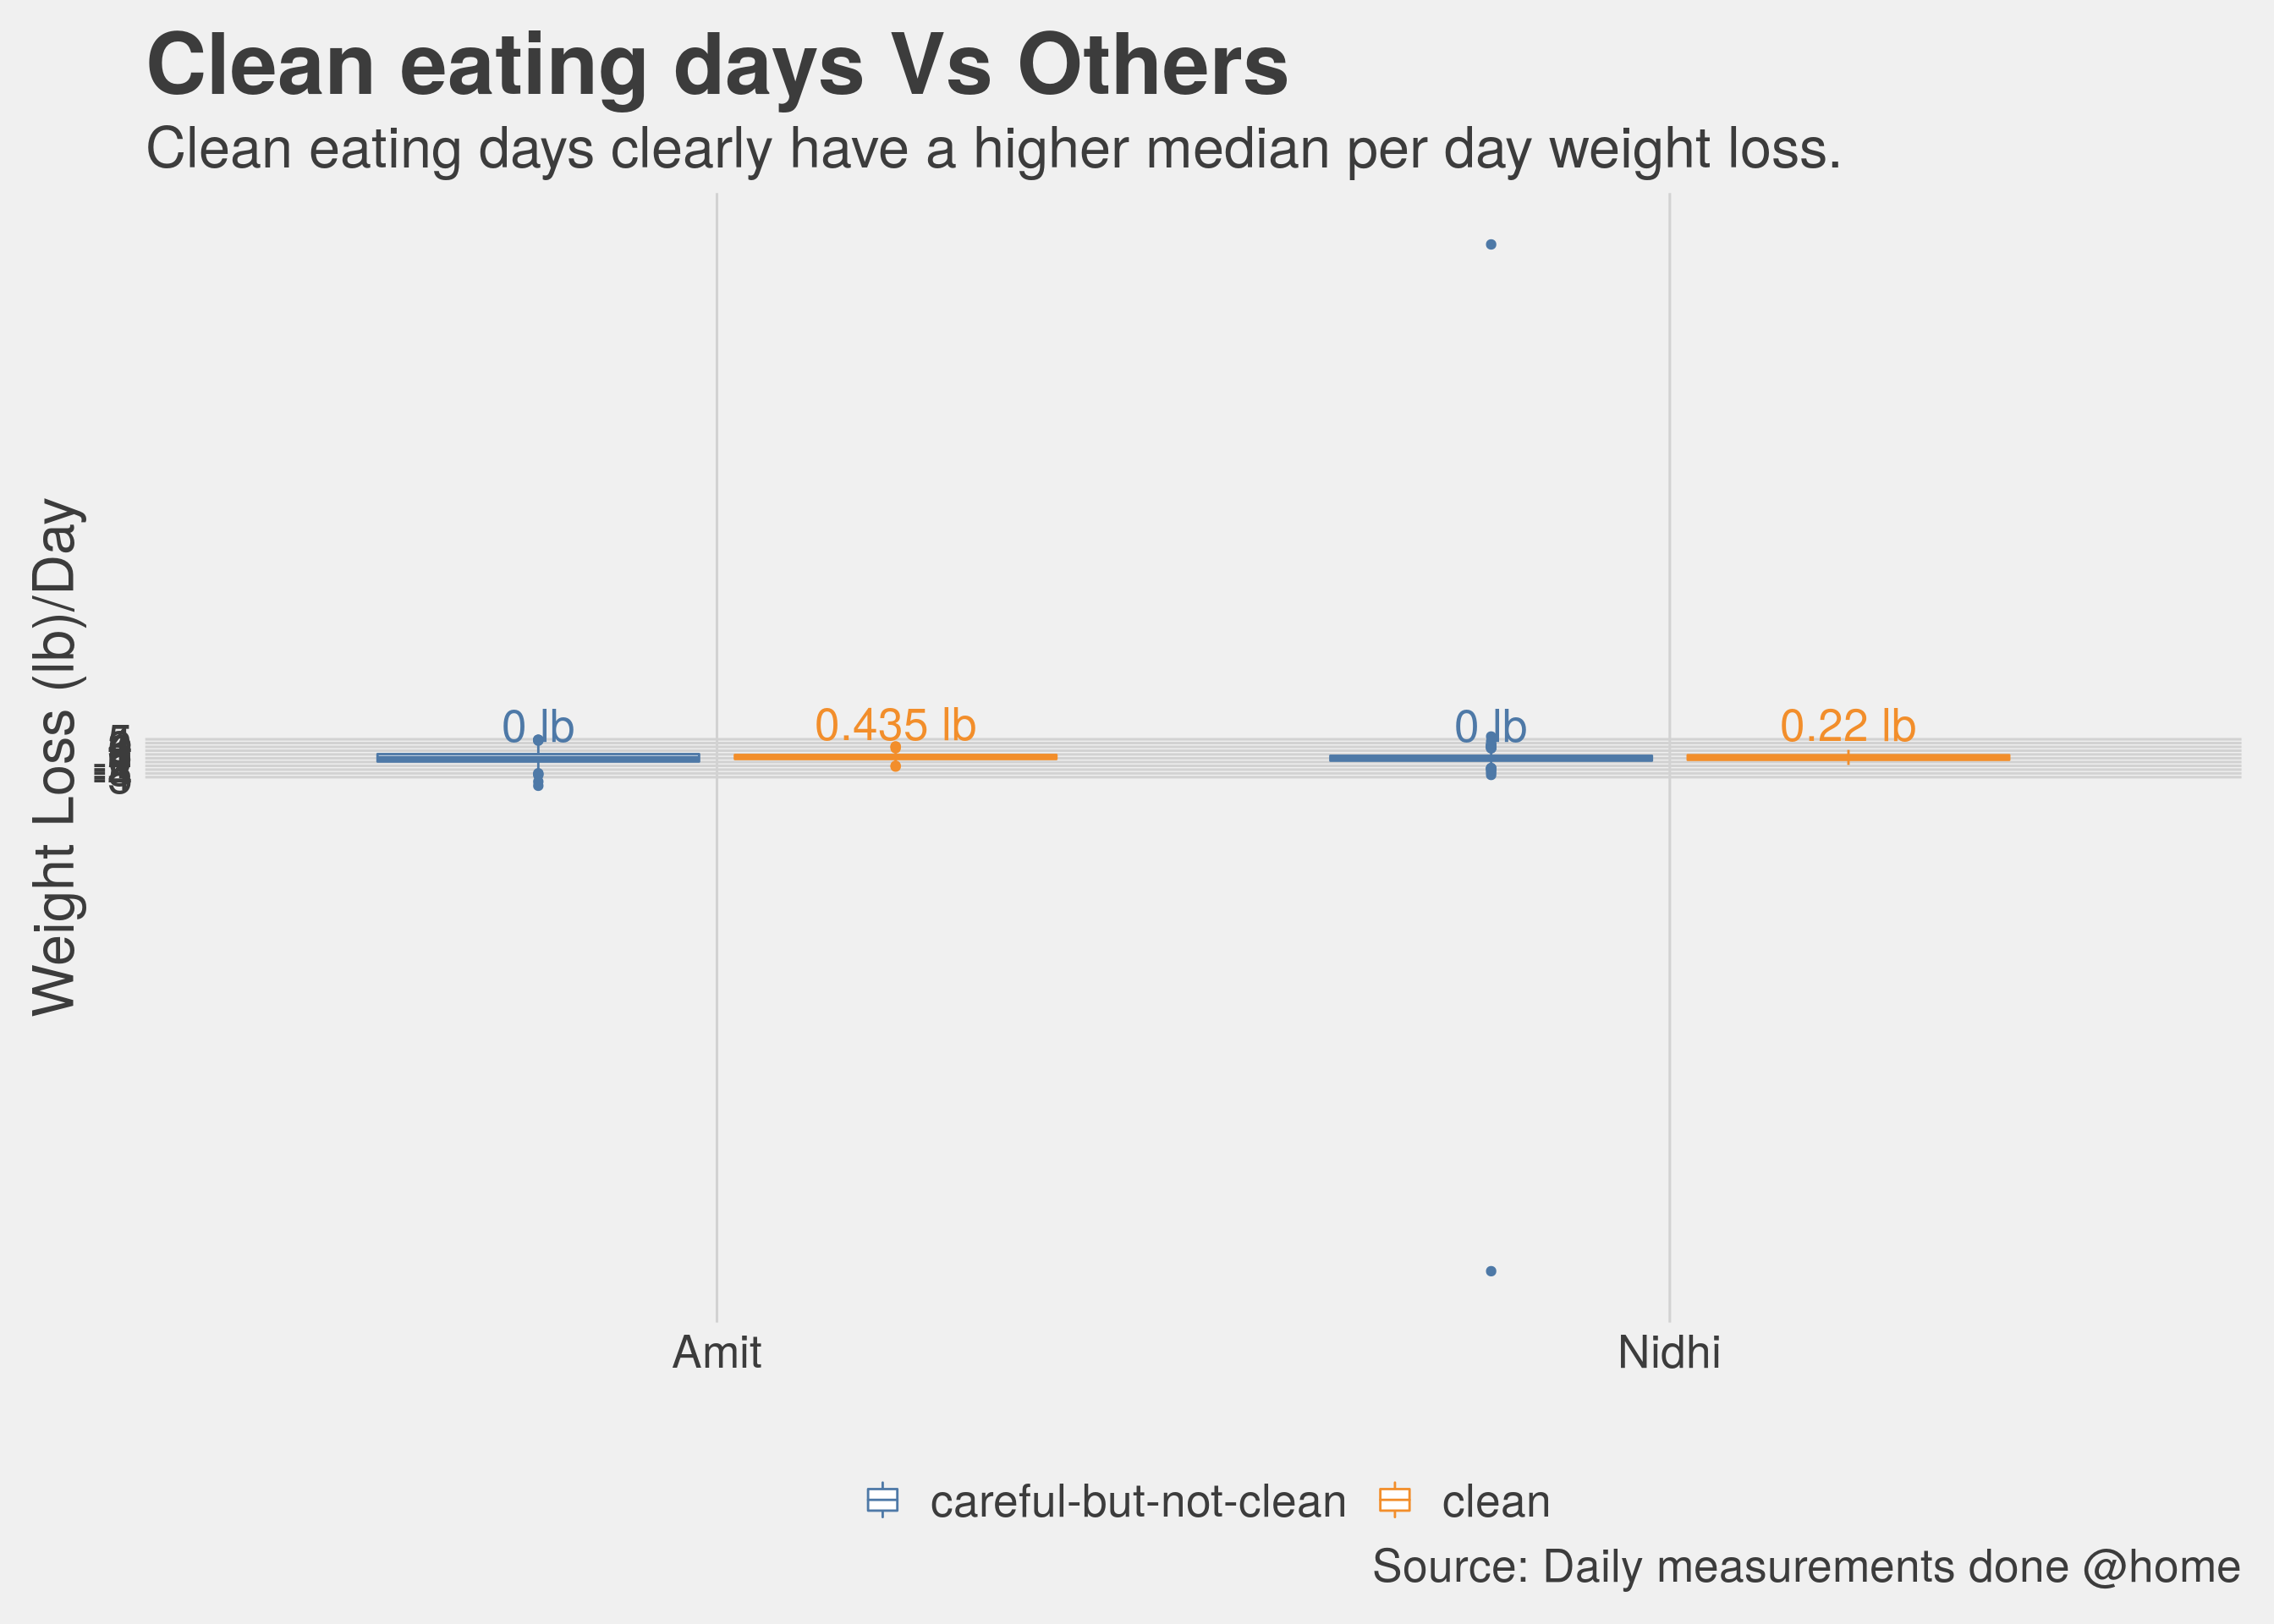
\includegraphics{bookdownproj_files/figure-latex/unnamed-chunk-6-1.pdf}

Here is another chart that compares the weight loss during clean eating
and non-clean eating days. Note that even when we were not doing clean
eating we were still careful about what we were eating (in other words
we were not gorging on Pizzas and butter chicken, soft and hard drinks
were still completely off limits).

The chart shows a boxplot representing the spread of the weight loss per
day during clean eating periods and non-clean eating periods. The
horizontal line inside the box represents the median value of the
distribution. For example, I lost at least 0.435 lb per day on 50\% of
the days during clean eating whereas I only lost at least 0.005 lb on
50\% of the days during non-clean eating period. The data for this chart
includes both clean eating periods over a timespan from 2020-02-17 to
2020-09-08.

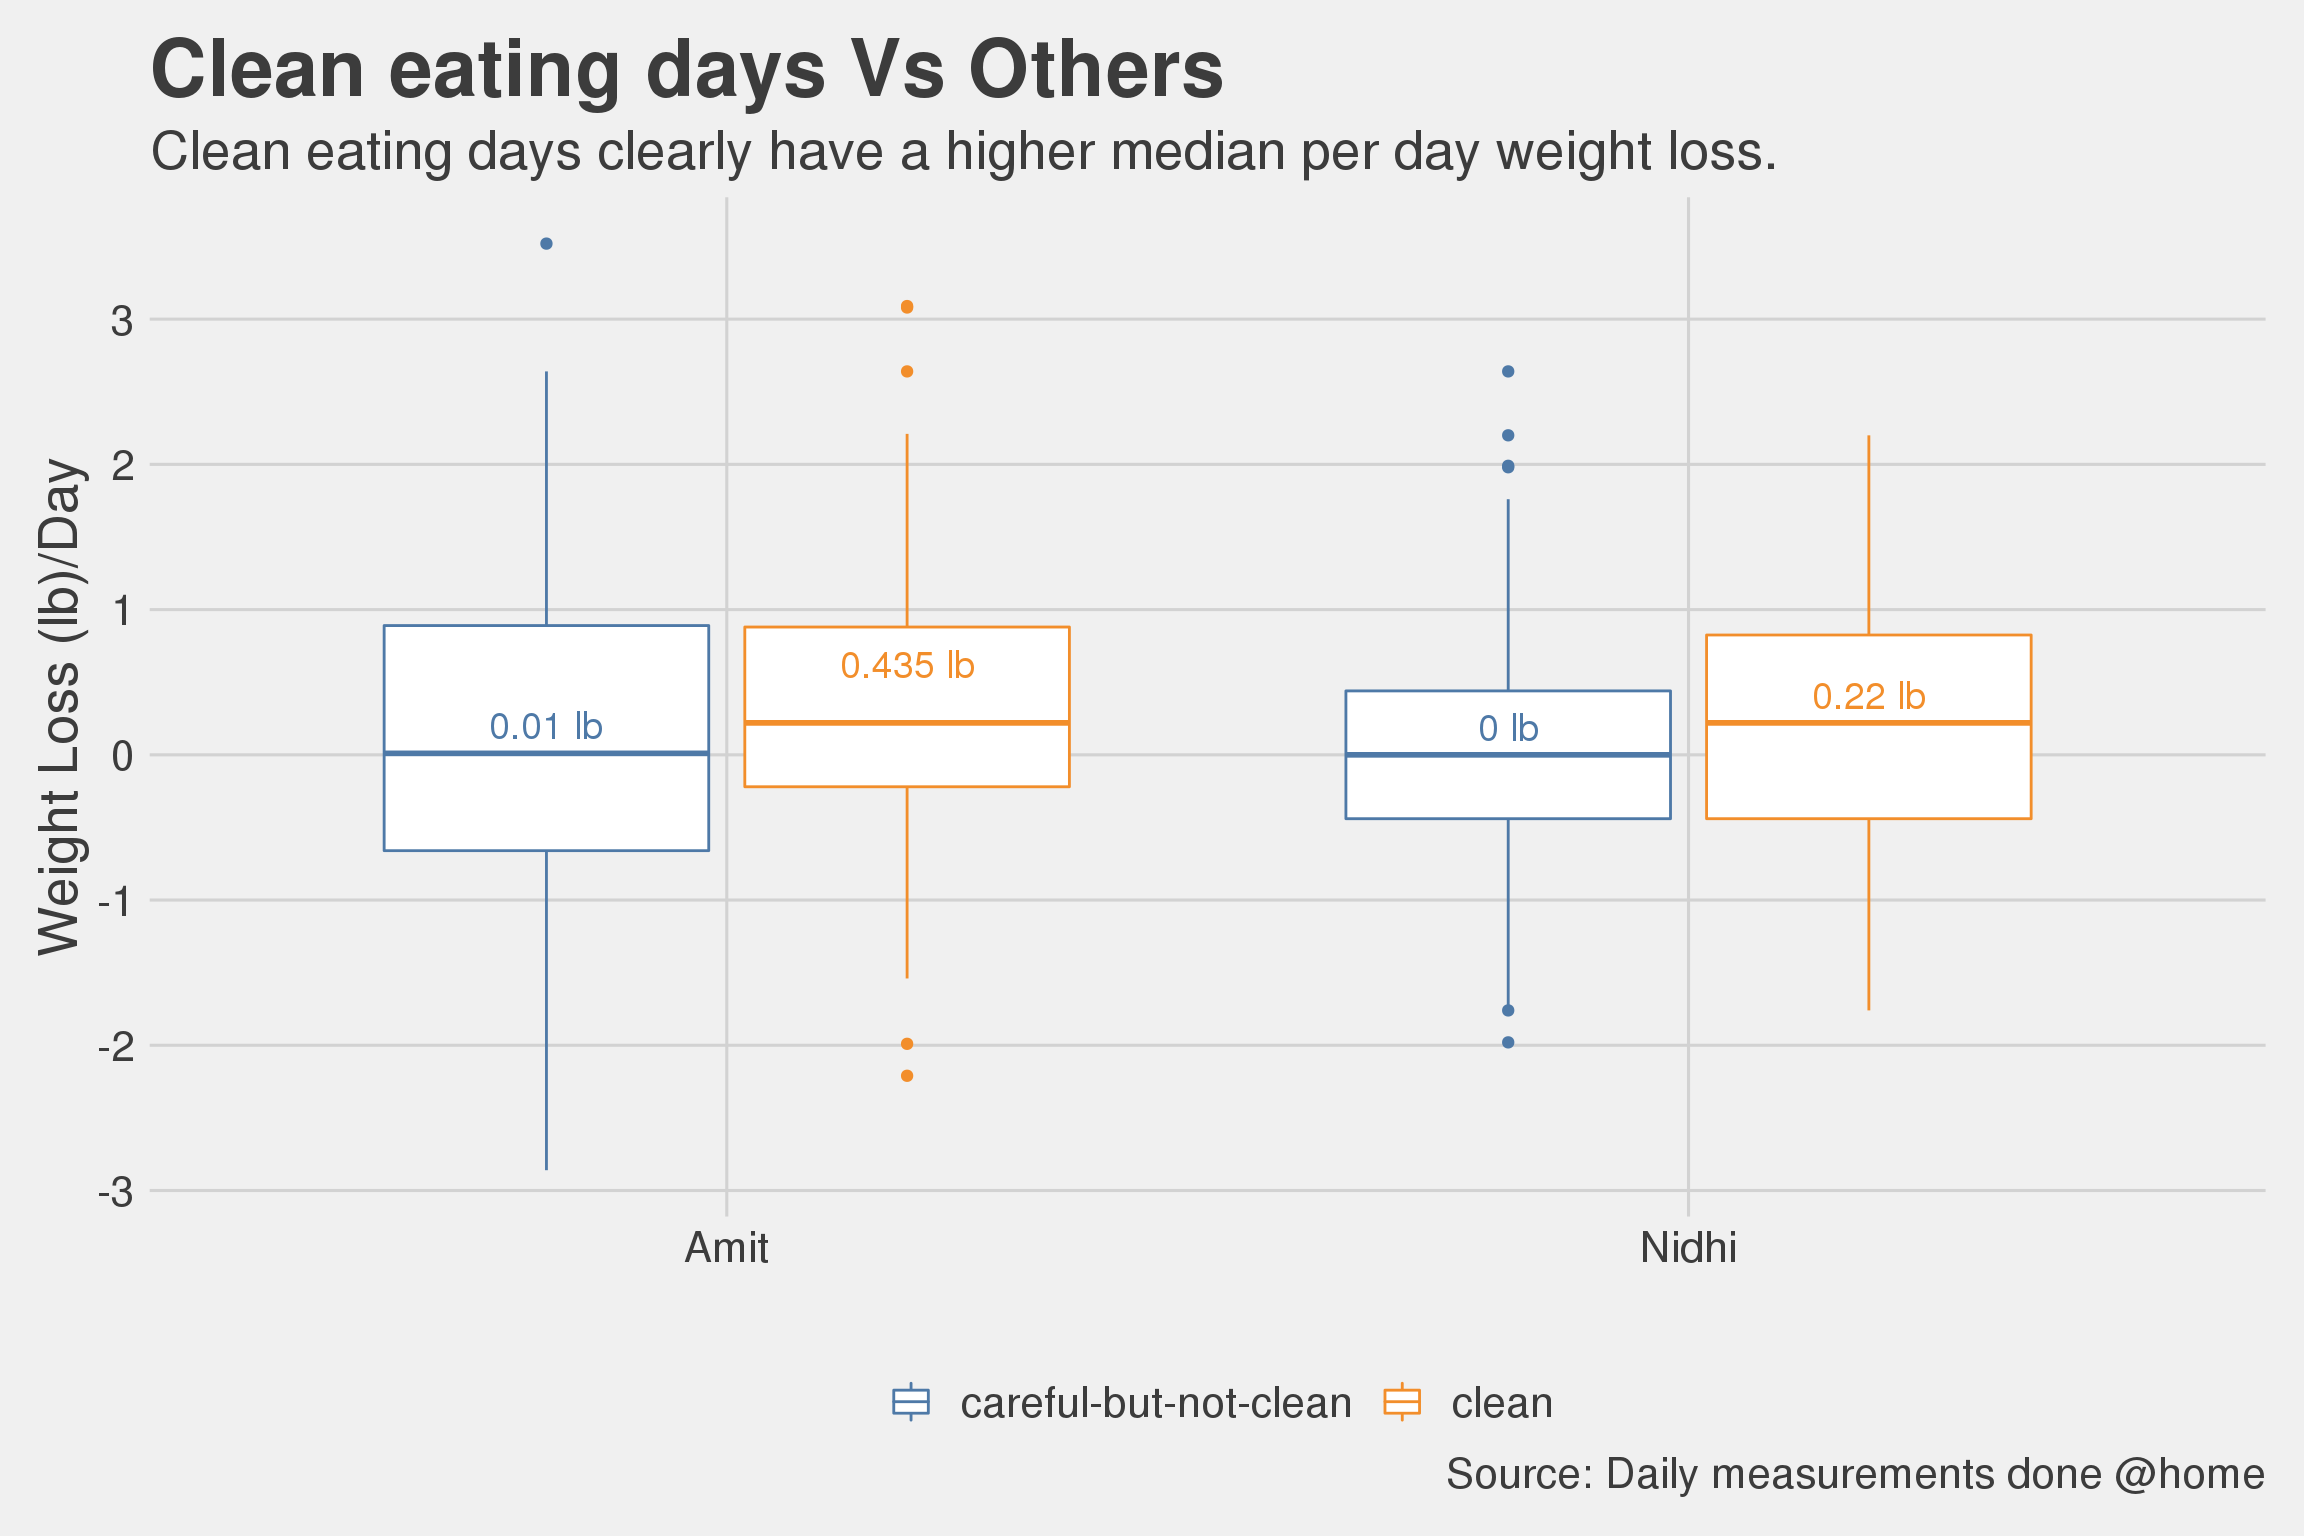
\includegraphics{bookdownproj_files/figure-latex/unnamed-chunk-7-1.pdf}

\section{Is the 30 day challenge
hard?}\label{is-the-30-day-challenge-hard}

I will be blunt here, it is not as hard, certainly I did not feel it
was, BUT tedious and tiresome is how i would describe it. The fact that
there isn't a restriction on eating vegetables or fruits makes it easier
than other diet programs that I know of. It is a given that you are not
eating potato fries everyday for lunch or a mango for after dinner
dessert every night. What makes it hard is that after the first few days
the enthusiasam beings to wane and the new eating habits take some time
to become friendly. Once you adjust, both body and mind, to the new
eating regimen then it does not feel like a diet at all. It certainly
helps to have a goal in mind and keep reminding yourself why are you
doing this.

For me, I think after two weeks or so, I could certainly start feeling
the benefits, I felt lighter, more energetic (no mid afternoon energy
crashes), better quality of sleep, just overall lot of positives. While
all this is happening, an interesting incident occured. We had to be at
a friend's place for a birthday dinner, the host was gracious enough to
prepare some salads for us and we also took our own food with us. Midway
through the party, i suddenly started feeling uncomfortable. The smell
(aromas) of all the food and more so the alcoholic drinks made me feel
nauseous, I felt like throwing up. Fortunately I did not throw up and we
had a very enjoyable evening other than those 30 minutes. I reflected on
that later, I was totally fine when we were back home, totally fine the
next day as well. It must be that 3 weeks into clean eating the internal
circuitery in my body had maybe begun to rewire itself, or so I thought.

Another thought that often came to my mind was that good food is a
source of happiness, of joy. The sweet gulps of the
\href{https://en.wikipedia.org/wiki/Lassi\#Mango_lassi}{mango lassi}
soothe the soul, the tangy and crisp
\href{https://en.wikipedia.org/wiki/Panipuri}{Gol Gappe} tickle the
brain, a \href{https://en.wikipedia.org/wiki/Paratha}{mooli or carrot or
onion paratha} satiate the stomach like nothing else, and what even
comes close to a
\href{https://en.wikipedia.org/wiki/Butter_chicken}{butter chicken}?
This is all true, however, food does not have to be the ``only'' source
of happiness. There is happiness to be derived from good health, from
feeling light, awake and agile throughout the day. A round of vigorous
exercise resulting in a body drenched in sweat and a rush of endorphins
is also happiness. Give it a chance, it will not disappoint you.

\section{What happens after the 30 day
challenge?}\label{what-happens-after-the-30-day-challenge}

Several people have asked me, ``like other diets, do you go back to your
old weight after you stop clean eating?''. My answer is ``yes, most
certainly'' and this should not be a surprise. While I would not call
clean eating a ``diet'', it is certainly accurate to say that there is
no such thing as a ``one time fix''. If you want the effects to be
permanent then the lifestyle changes also have to be permanent, there
are no quick fixed. I have often heard in other contexts that being
fit/healthy/strong requires a lifestyle change. It certainly does. Does
it mean we can never eat unhealthy food, no it does not mean that, it
means that you first become healthy enough to allow your body the
occasional indiscretions and then the morning after you go back to
eating healthy and doing excercise.

As our 30 day challenge was coming towards an end I was very much
looking forward to eating a lot of fried Indian delicacies, all in one
meal. I did that, probably having deprived myself a lot, went a tad bit
overboard. The results were not pleasant. After about an hour, i started
feeling miserable. I felt bloated, tired, lethargic and sleepy. For a
moment I could not understand what was happening, sounds like an
exaggeration but I had almost forgotten what it felt like to overeat.
Nidhi then pointed out it was probably because of all the food i ate,
that made total sense. I felt so full, i did not eat anything in the
afternoon, nothing in the evening for dinner either. Next morning i felt
much better. This was my body's way of telling me that you do this again
and I am going to react to this as if there is an alien invasion and the
planet is in danger. Make no mistake, I have not stopped eating that
food, I just eat smaller portions of it because I realize that what
follows after the 30 minutes of pleasure is 24 hours of unpleasantness.

\chapter{Exercise: Putting in the hard
yards}\label{exercise-putting-in-the-hard-yards}

\chapter{What did we accomplish?}\label{what-did-we-accomplish}

I have said this earlier in this book, my initial goal for meeting with
a trainer and going to the gym was to lose weight, but as we started
sweating it out I realized that we were getting a lot more out of this
exercise and clean eating regimen than just a lighter body. Even so,
weight loss and overall getting the body in a better shape are important
goals, so how did we fare on these?

\captionsetup[table]{labelformat=empty,skip=1pt}

\begin{longtable}{cll}
\caption*{
\large \textbf{Important Metrics}\\ 
\small Key data points that describe the journey\\ 
} \\ 
\toprule
Metric & Amit & Nidhi \\ 
\midrule
Days since start & 204 & 204 \\ 
Days taken to lose last 10 pounds & 56 & 84 \\ 
Starting Weight (lb) & 251.33 & 151.9 \\ 
Current Weight (lb) & 203.49 & 130.07 \\ 
Total weight loss (lb) & 47.84\textsuperscript{1} & 21.83\textsuperscript{2} \\ 
Best Weight loss month & May, 8.38 lb & Mar, 6.18 lb \\ 
\bottomrule
\end{longtable}

\vspace{-5mm}

\begin{minipage}{\linewidth}
\textsuperscript{1}19.03\% of the starting body weight. \\ 
\textsuperscript{2}14.37\% of the starting body weight. \\ 
\end{minipage}\begin{minipage}{\linewidth}
Source: Daily measurements done @home\\ 
\end{minipage}

\section{Percentages are revealing}\label{percentages-are-revealing}

So net-net in about 7 months, I lost about 20\% of my body weight and
Nidhi lost about 15\%. Not too bad. In terms of how far we have
progressed compared to the goals we started with, I have some more miles
to go while Nidhi is almost there.

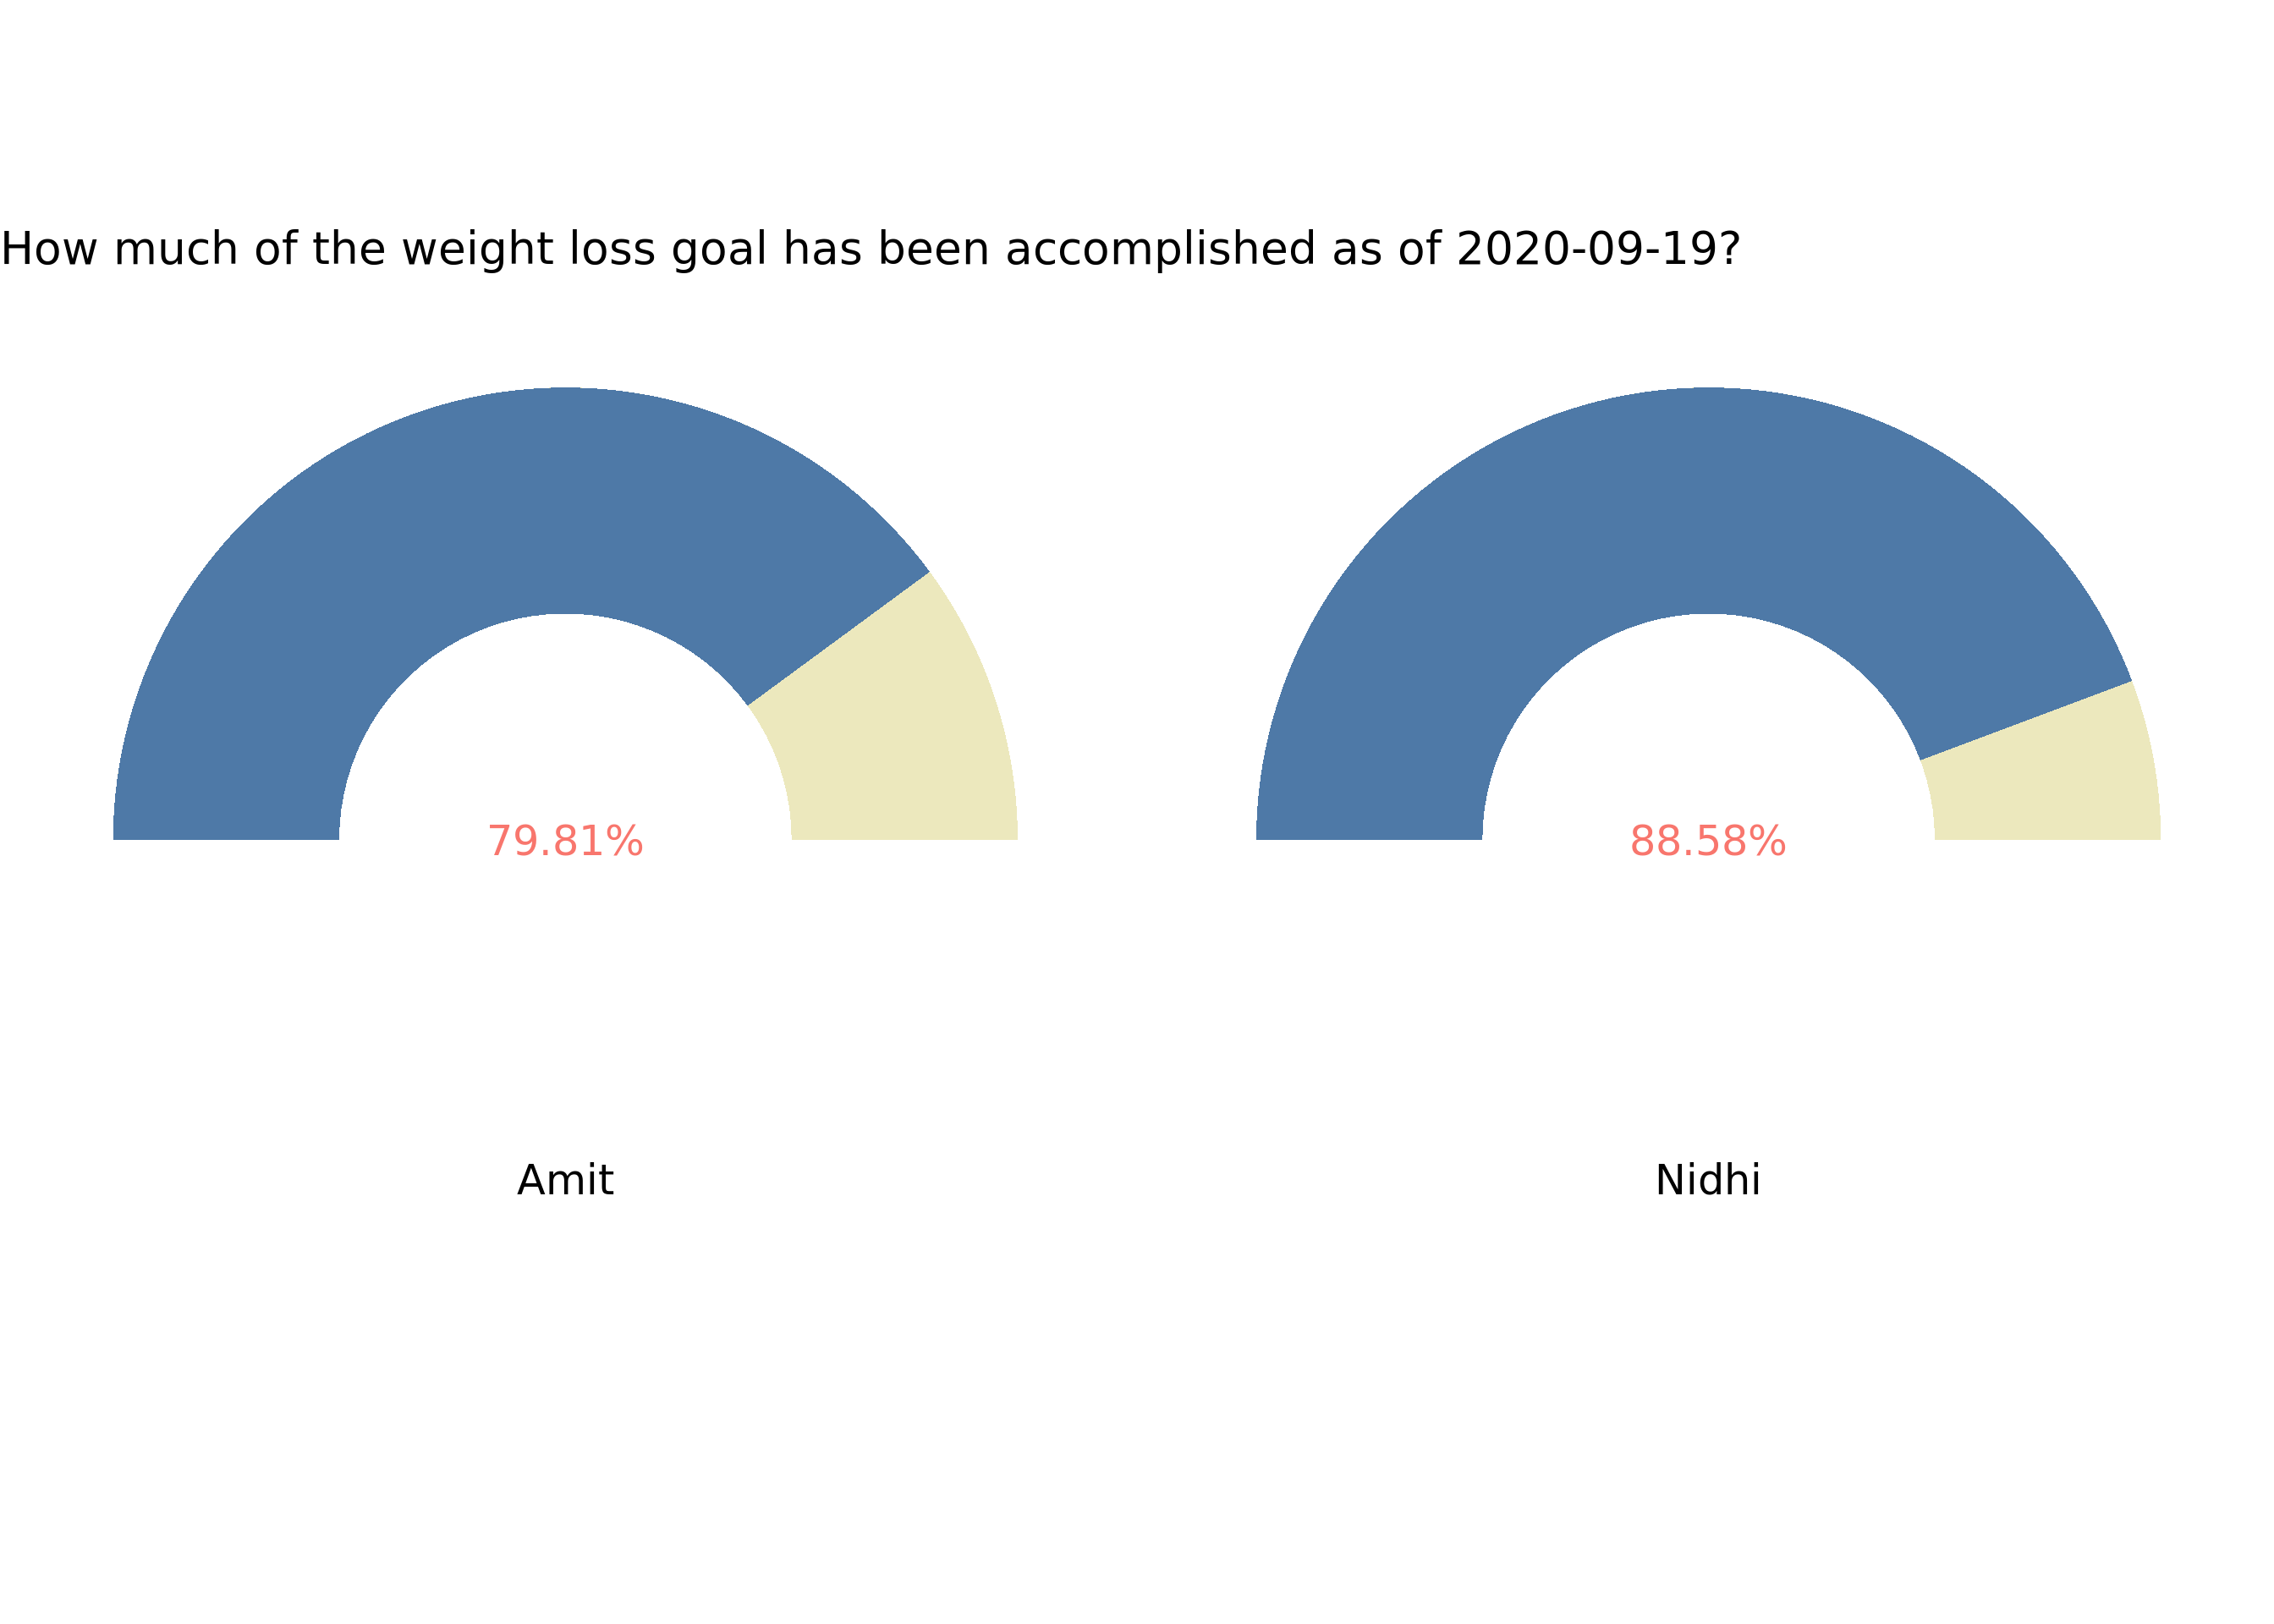
\includegraphics{bookdownproj_files/figure-latex/unnamed-chunk-10-1.pdf}

\section{Changes in other biometrics}\label{changes-in-other-biometrics}

Along with the body weight, other metrics also saw significant change.
This is seen in the following charts. BMI is widely used (I suppose
accepted as well) measurement to determine if someone is healthy, obese
or overweight. We saw reduction in BMI as well which as expected is
correlated to the reduction in weight. NIH guidelines for BMI are
available
\href{https://www.nhlbi.nih.gov/health/educational/healthdisp/pdf/tipsheets/Are-You-at-a-Healthy-Weight.pdf}{here}
for reference.

All measurements in the charts below were done automatically as part of
the daily metrics measured by the scale and synched with our phone. This
made it really easy to collect and analyze this data.

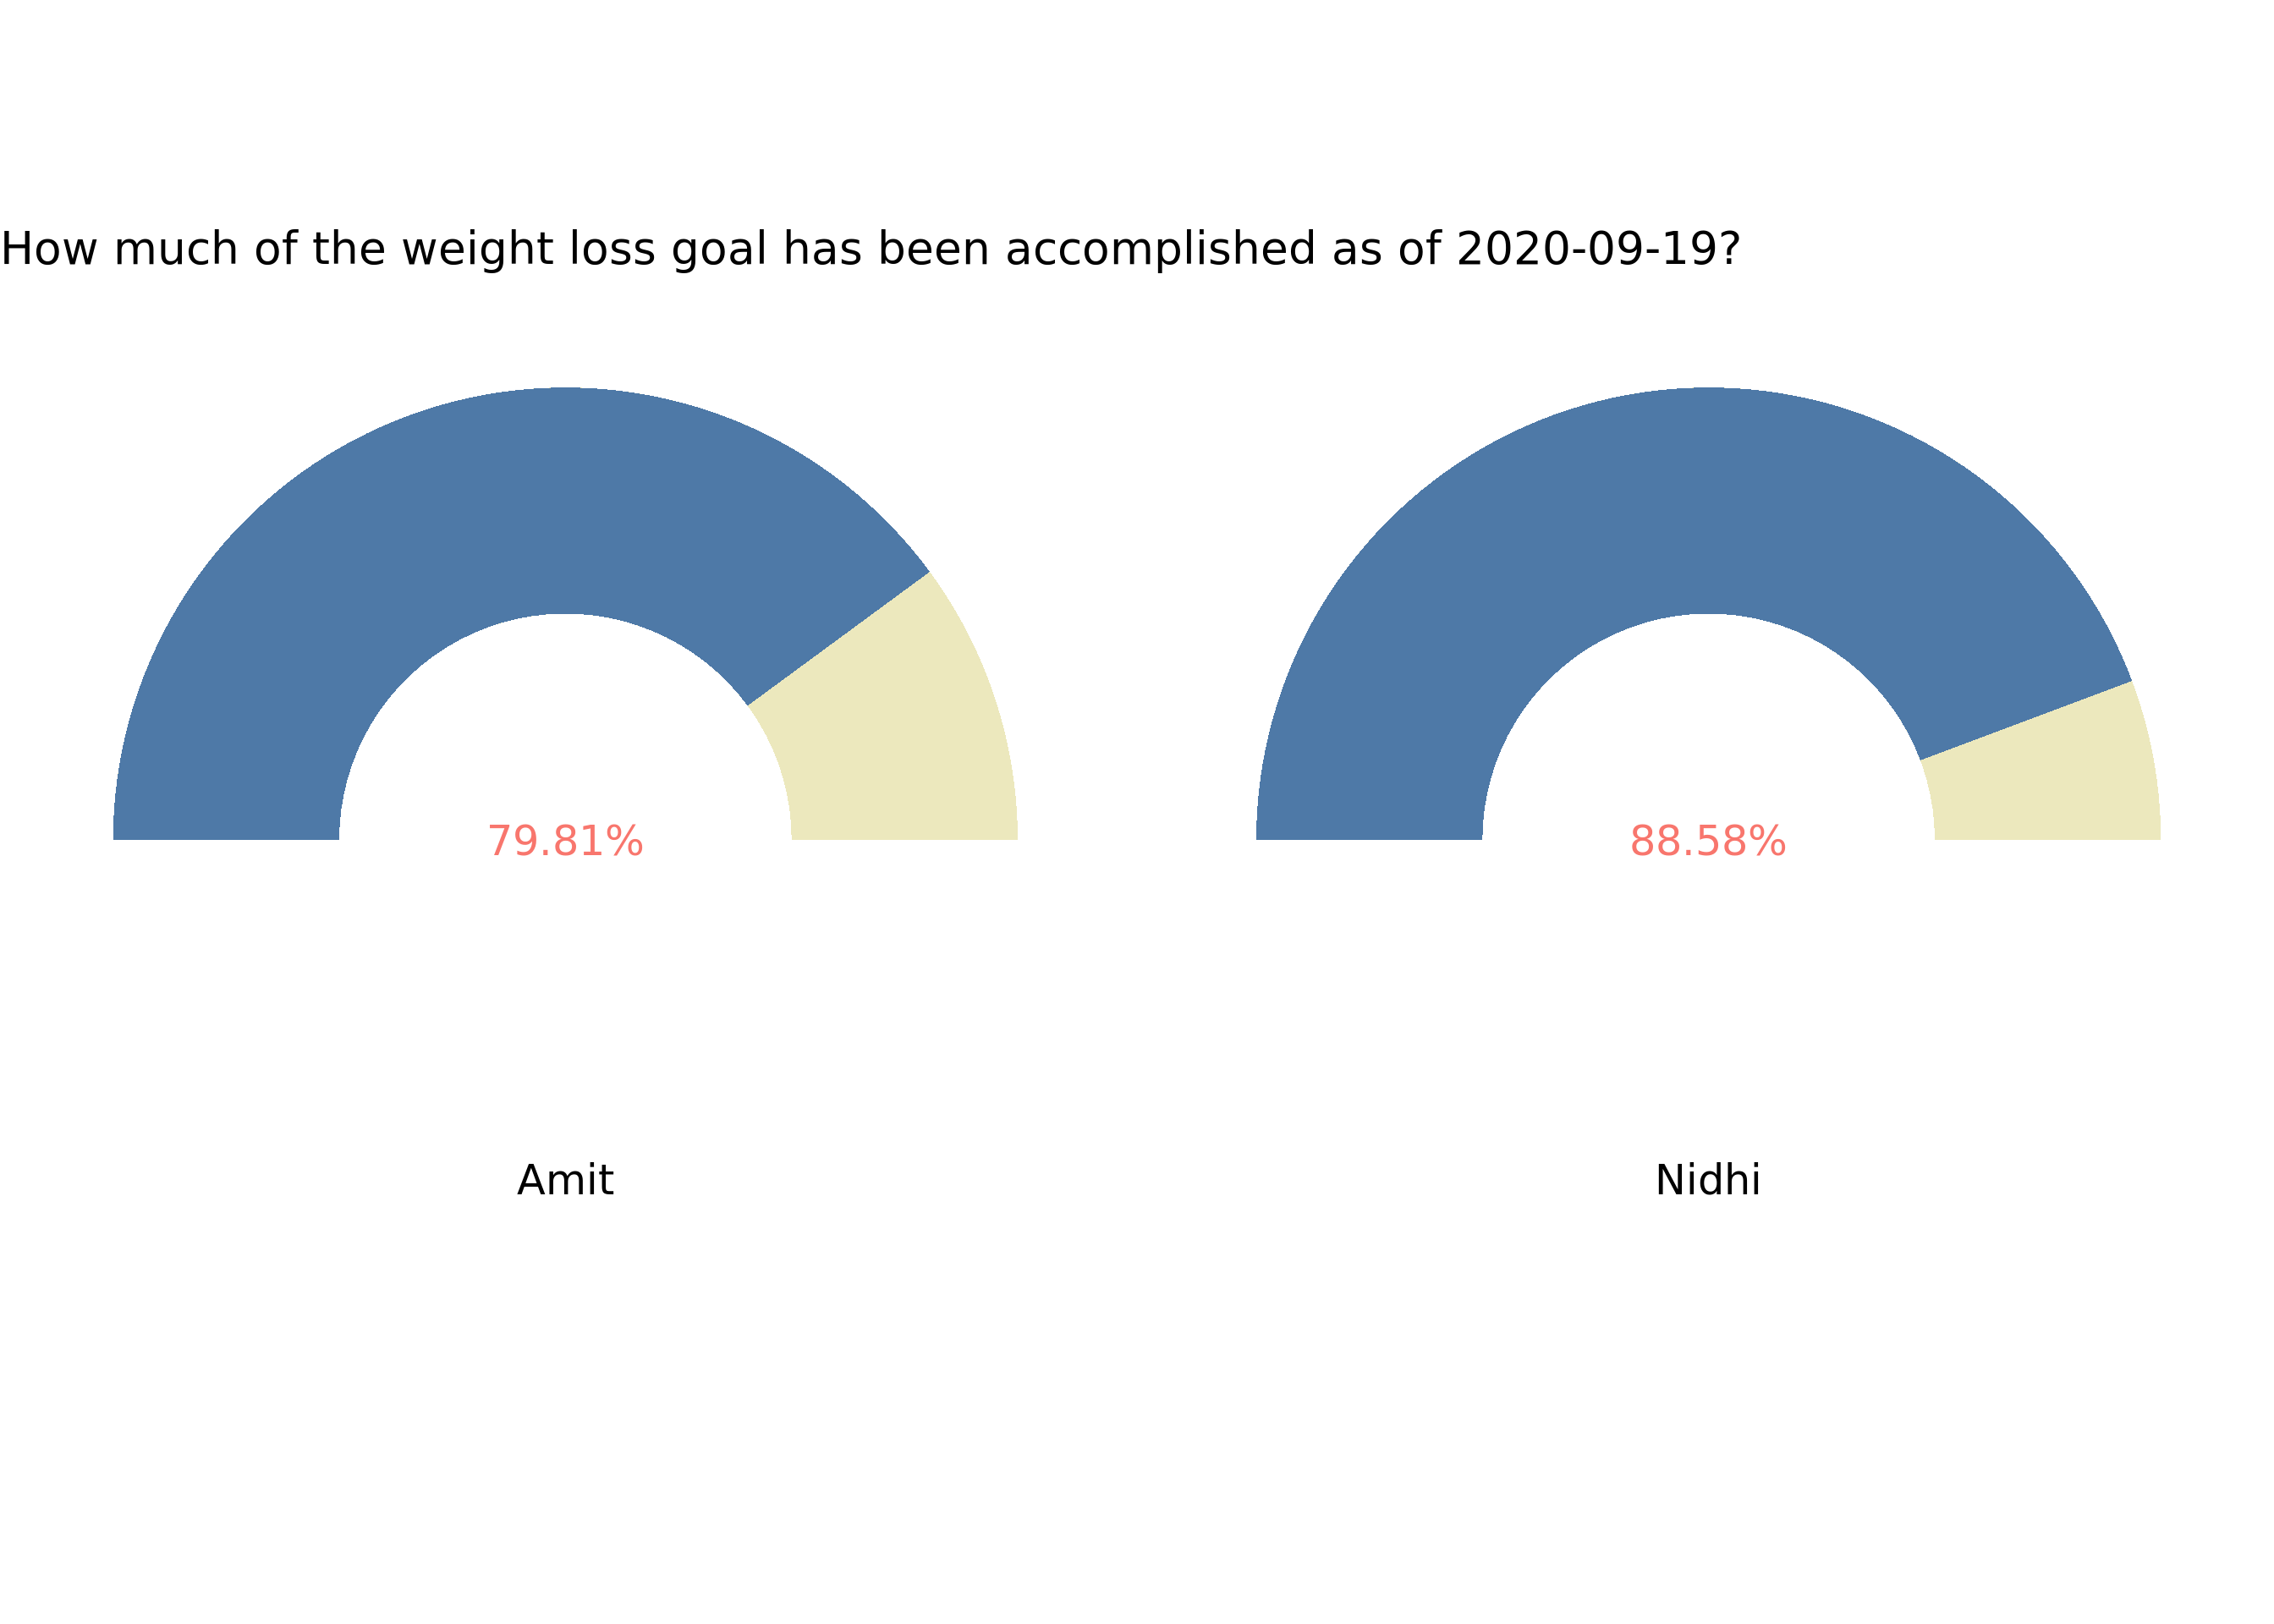
\includegraphics{bookdownproj_files/figure-latex/unnamed-chunk-11-1.pdf}

\section{Body measurements}\label{body-measurements}

Weight and BMI is not the only metric we tracked, these metrics are
often times all we think in terms of measuring but there is more. Just
as the proof of the pudding is in the eating, the proof of the weight
loss is in the wearing (of clothes). As we kept on making progress in
our journey, the clothes started fitting well at first, then getting
loose and the finally it reached a point where most of our old clothes
were just too big and this necessitated a wardrobe refresh. A happy
problem to have.

We tracked this by doing body measurements once every few months. The
charts below have a story to tell.

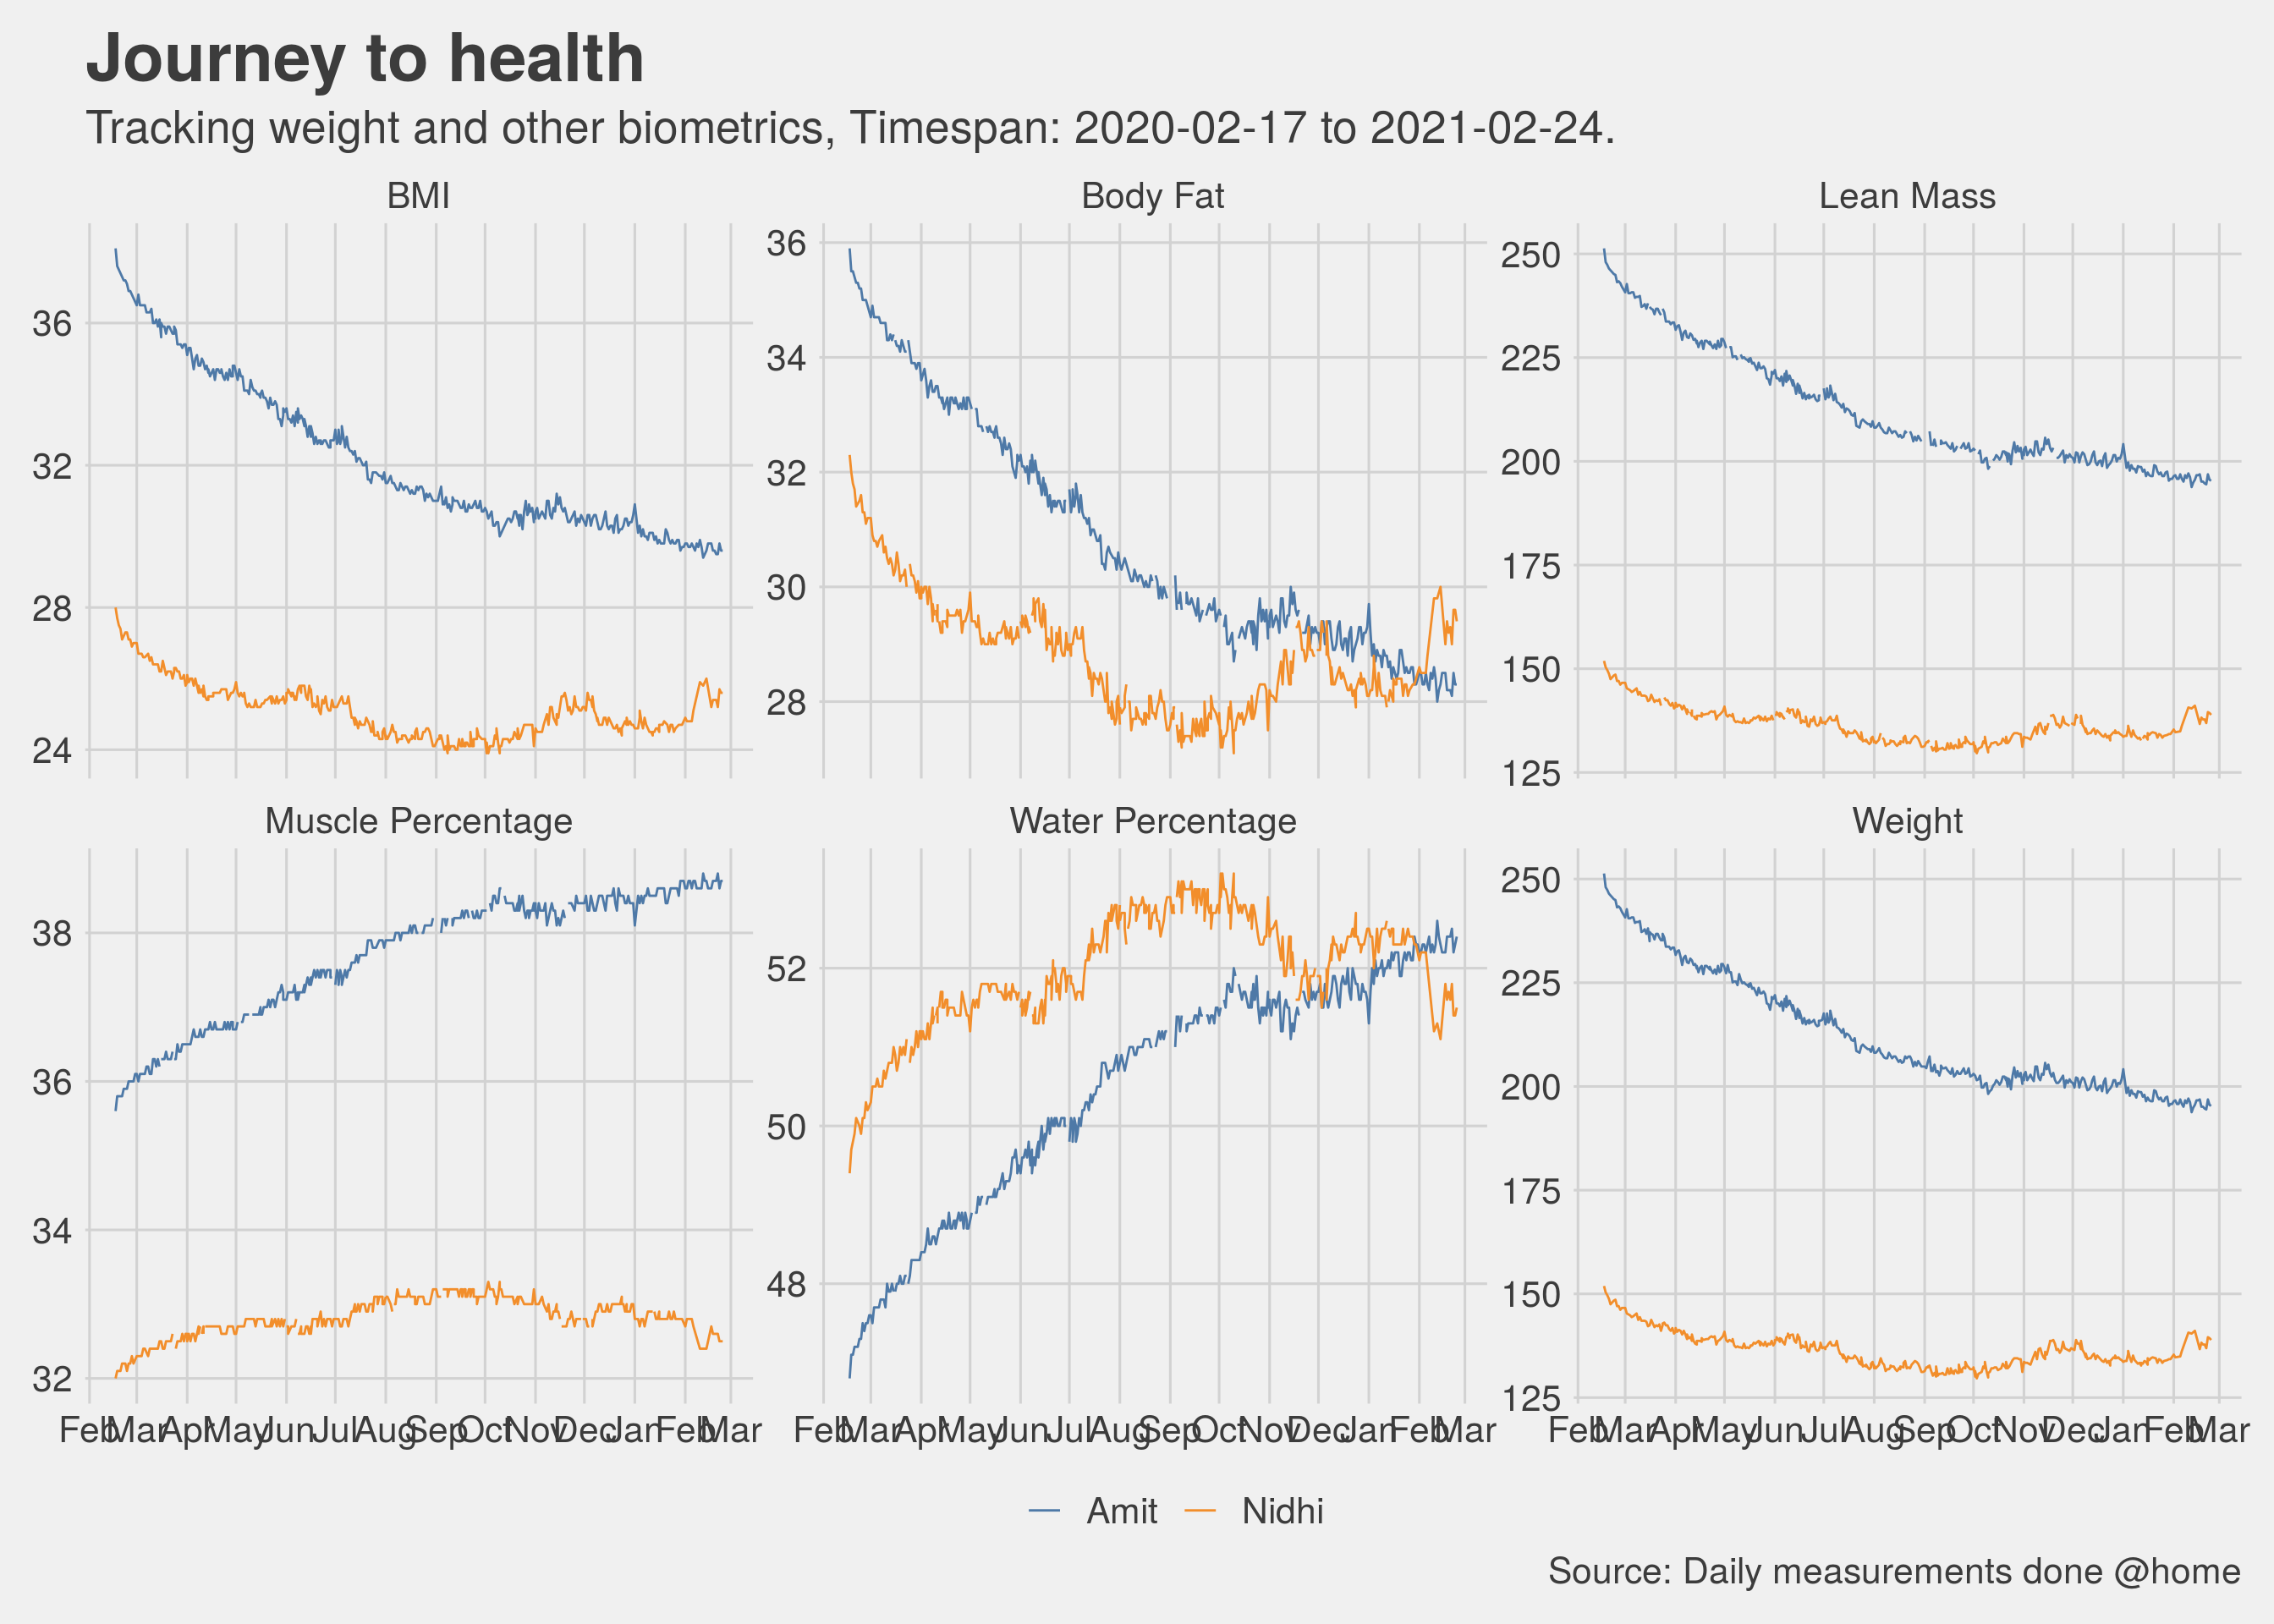
\includegraphics{bookdownproj_files/figure-latex/unnamed-chunk-12-1.pdf}

\section{A forecast and a promise}\label{a-forecast-and-a-promise}

As we were going through this journey, I was very eager to apply some
forecasting and determine if we could project a reasonable date when we
would be able to meet our weight loss target. As much as this book is
not just about weight loss, there is no denying the fact that it was one
of the most (if not the most) tangible outcome we were tracking towards.

Once we had collected a reasonable amount of data, I used standard
timeseries forecasting techniques to determine how our weights would
look say 30, 90 or 180 days from the current date. I used the
\href{https://facebook.github.io/prophet/\#:~:text=Prophet\%20is\%20a\%20procedure\%20for,daily\%20seasonality\%2C\%20plus\%20holiday\%20effects.\&text=Prophet\%20is\%20robust\%20to\%20missing,and\%20typically\%20handles\%20outliers\%20well.}{Prophet}
package from Facebook AI Research
(\href{https://github.com/facebookresearch}{FAIR}) to do the timeseries
forecast. The results are presented below. This forecast was done on
August 16, 2020 and as per this forecast we should be able to achieve
our target weight in early October for Nidhi and mid-December for me.

Once we had these forecasted date and the plots created, we started
monitoring very closely if our daily weight measurements were within the
range of errors as shown in these plots. Some days the weight did creep
out of the error limits but then it served as a nice tool to keep us
honest, so in a manner of speaking we knew how much we could deviate. So
if an Indian takeout dinner one evening did set us back, we knew we had
to make up for it in the next few days to come back within acceptable
range. So far it seems the projects are holding up reasonably well. If
nothing else, it provides certain guard rails to not let one go
completely off track. The promise still is, if we keep doing what we
have been diligently doing, we should be able to achieve our goals
around, if not exactly on, the forecasted date. It is important to
mention here, this simple forecast is considering the weight loss as a
univariate timeseries i.e.~single variable timeseries, we know it is
much more complicated than that. The premise is that all exogenous
factors remaining the same, this forecast should hold up.

\hypertarget{htmlwidget-1d91bf123804b10073f4}{}

\hypertarget{htmlwidget-a34476f2f82484e0b26e}{}

\chapter{Do I Need a Trainer?}\label{do-i-need-a-trainer}

\chapter{Time Restricted Eating}\label{time-restricted-eating}

\chapter{Other Topics}\label{other-topics}

\end{document}
